\documentclass{llncs}

\usepackage{hyperref}
\usepackage{url}
\pagestyle{plain}
\usepackage{threeparttable}
\input{math_commands.tex}

%\usepackage[latin9]{inputenc}
%\usepackage[T1]{fontenc}
\usepackage{float}
\usepackage{wrapfig}
\usepackage{amsmath}
\usepackage{amssymb}
\usepackage{graphicx}
\usepackage{subcaption}
\usepackage{tabularx}
\captionsetup{compatibility=false}
% \usepackage{esint}
\usepackage{array}
\usepackage{epstopdf}
\usepackage{placeins}
\usepackage{pgfplots}
\usepackage{url}
\usepackage{tikz}
\usepackage{calc}
\usepackage{array}
\usepackage[linesnumbered,ruled,vlined]{algorithm2e}
\usetikzlibrary{positioning, arrows.meta,calc}

%%%%%%%%%%%%%%%%%%%%%%%%%%%%%%%
%%%%%%%%%%%%%%%%%%%%%%%%%%%%%%%


\newcommand{\vW}{\boldsymbol{W}}

\newcommand{\val}{{\textrm{value}}}
\newcommand{\Val}{{\textrm{value}}}
\newcommand{\MILP}{{\textrm{MILP}}}
\newcommand{\LP}{{\textrm{LP}}}
\newcommand{\Improve}{\mathrm{Improve}}
\newcommand{\Utility}{\mathrm{Utility}}
\newcommand{\Sol}{\mathrm{Sol}}
\newcommand{\sol}{\mathrm{sol}}

\newcommand{\UB}{\mathrm{UB}}
\newcommand{\LB}{\mathrm{LB}}
\newcommand{\ub}{\mathrm{ub}}
\newcommand{\lb}{\mathrm{lb}}
\newcommand{\B}{\mathrm{B}}
\usepackage{amsmath, amssymb, amsfonts}


\newcommand{\ReLU}{\mathrm{ReLU}}

\newcommand{\CMP}{{\textrm{CMP}}\ }


\newcommand{\toolname}{Hybrid MILP}


\title{I Compensate, therefore I Am \\ (accurate for DNN verification)}
\date{}

\begin{document}
	


\section{Introduction}

Deep neural networks (DNNs for short) have demonstrated remarkable capabilities, achieving human-like or even superior performance across a wide range of tasks. However, their robustness is often compromised by their susceptibility to input perturbations \cite{szegedy}. This vulnerability has catalyzed the verification community to develop various methodologies, each presenting a unique balance between completeness and computational efficiency \cite{Marabou,Reluplex,deeppoly}. This surge in innovation has also led to the inception of competitions such as VNNComp \cite{VNNcomp}, which aim to systematically evaluate the performance of neural network verification tools. Among them, NNenum \cite{nnenum}, Marabou \cite{Marabou,Marabou2}, and PyRAT \cite{pyrat} MnBAB \cite{ferrari2022complete}, built upon ERAN \cite{deeppoly} and PRIMA \cite{prima}; and $\alpha,\beta$-CROWN \cite{crown,xu2020fast}, 
%the winner of the last 4 VNNcomp, benefiting from 
based on branch-and-bound based methodology \cite{cutting,BaB}.

These tools %benchmarks usually 
focus on {\em local} robustness, i.e. given a DNN, an image and a small neighborhood around this image, is it the case that all the images in the neighborhood are classified in the same way by the DNN? The neighborhood is provided by a maximal perturbation of the input image, often an 
$L_\infty$-perturbation, i.e. every subpixel of the input image can vary in a very small range, typically $\frac{2}{255}$ (that is 2 levels of grey/blue/red/green). 
Although it is not necessarily the most meaningful perturbation,
$L_\infty$ is the usual choice because it is perfectly linear and specifies 
subpixel perturbations independantly, which is easier to verify. 
Importantly, these verification tools for local robustness are too computationally-intensive to be used in a real-time decision making pipeline: considering an autonomous car with a video feed from the dashboard, 
images of the feed cannot be certified robust in few ms on embedded hardware to e.g. skip non-robust images and only consider certified robust images.
% for the decision-making process.

\smallskip

In this paper, we consider {\em global} robustness, that is we do not restrict the certification process to the neighborhood of a fix input. We follow a two steps procedure. 
The first step, performed offline once, computes global bounds on the shift between 
output values of different decision classes due to the perturbation, close to \cite{vhagar}. That is, considering decision classes $C$ and $D$ and perturbation $\varepsilon$, compute an 
upper bound $\bar{\beta}^\varepsilon_{C,D}$ of $\max_{I,I', |I-I'| \leq \epsilon}(value_{I}(C) - value_{I}(D) + value_{I'}(D) - value_{I'}(C))$, where $value_{J}(X)$ is the output value of class $X \in \{C,D\}$ for input image $J \in \{I,I'\}$. %Notice that as $I,I',C,D$ have symetrical roles, we can choose $\beta^\varepsilon_{D,C} = \beta^\varepsilon_{C,D}$. Also, as $I,I'$ have symetrcal role, the minimum value is exactly $-$ the maximum value. 
%Hence, if we have $n$ decision classes, we only have to compute $n (n-1)/2$ bounds. 
Bound $\bar{\beta}^\varepsilon_{C,D}$ is computed offline once for a DNN, 
and it is valid over the whole input space; compared with $k$ calls to 
{\em local} robustness, once for each of the $k$ input images, with results only valid for these $k$ images.

The second step is real-time, being performed with the DNN inference of the image $I$ considered: it suffices to consider the class $C$ with the highest output value $value_{I}(C)$, and check whether for every other class $D \neq C$, 
$value_{I}(C) - value_{I}(D) > \bar{\beta}^\varepsilon_{C,D}$. 
If this is the case, then we are certified that image $I$ is robust for perturbation $\varepsilon$, because $\varepsilon$-perturbed image $I'$ could at most get  $value_{I'}(D) \leq \bar{\beta}^\varepsilon_{C,D}  - (value_{I}(C) - value_{I}(D))  + value_{I'}(C) < value_{I'}(C)$, hence $C$ is also the predicted class for image $I'$. This typically needs a couple of tens CPU instructions, which can be performed under 1ms (mili-second) on a single CPU core. If the image is not certified robust, one could either skip image $I$ (in a video feed), or use safer degraded mode in the decision making process till a trustable robust image is received.


Our main contributions address the challenges to compute the {\em global bounds} $\bar{\beta}^\varepsilon_{C,D}$, for $C,D$ output neurons:
% for standard ReLU DNNs (e.g. \cite{vhagar}). Our findings can be extended to other activation functions, following similar extention by \cite{DivideAndSlide}:
%, with updated MILP models e.g. for maxpool:
\begin{enumerate}
	%\item  Our first contribution studies the {\em LP relaxation} of the exact MILP encoding of ReLUs. {\color{blue} We establish in Proposition \ref{LP} its equivalence with the so-called "triangular abstraction"}.
	
	\item We develop a novel {\em Diff MILP encoding} for the global robustness problem, %called the {\em "2v" model}, 
	where the variables are the values of the perturbed neurons, as well as the difference between the original and the perturbed neuron values (called the {\em diff variables}, introduced in \cite{diff}). We study and encode how the {\em diff variables} evolve after passing through a ReLU (Prop.~\ref{Prop2}), see Section \ref{s.diff}. 
	Compared with the {\em classical MILP model} \cite{MILP} employed in 
	\cite{vhagar,lipshitz,ITNE}, which considers the input and the perturbation but {\em diff variable}, we keep the same number of 2 binary variables per ReLU.
	%the results are more accurate for the same runtime.
	%the linear relaxation is much more accurate, as each {\em diff variable} can be bounded after a ReLU as a function of the value of the {\em diff variables} before the ReLU, whereas the linear relaxations of the classical model is extremely inaccurate, as the variables are independent of each other. This was observed in \cite{lipshitz,ITNE}, and constraints encoding
	%a part of the linear relaxation of our "2v" model were added explicitly. 
	%Experimentally, 
	However, our {\em Diff MILP model} is more efficient, one reason being 
	the accuracy of its linear relaxation.
	%The number of variables a priori doubles compared with local robustness, from each neuron value in the perturbed image to each neuron value in the perturbed image {\em and} in the original image, as the original image is no more fixed. 
	%Recall that the worst case complexity of MILP is exponential in the number of binary variables \cite{DivideAndSlide}. 
	%A straightforward MILP model would be to use the  for each of these variables, as in \cite{vhagar,lipshitz}. The main issue with the classical model is that its linear relaxations is extremely inaccurate, as the variables are independent of each other. Instead, we develop another exact MILP model, 

	\item Further, from the {\em Diff MILP model}, which is exact, 
	we develop two abstract MILP models, which are more efficient but also asymptotically less accurate than {\em Diff}. 
	Namely, the "2b+1" model, accurate on the {\em diff variables} but abstract on the perturbed variables; while the "1b" model has a unique binary variable per ReLU, only considering the {\em diff variables}.
	%\item We adapt the Solution Aware Scoring from \cite{ATVA25} to our novel MILP models, in order to select the most important ReLUs to be treated using complex binary variables, while less important variables are treated using linear relaxation. The chosen number of binary variables depends upon the complexity of the DNN as well as the targeted runtime.

   \item  In terms of perturbations, we consider conjunctions of $L_\infty$- and $L_1$-norms, which allow to accurately describe perturbations. For instance, "each subpixel is perturbed by at most $\frac{50}{255}$ ($L_\infty$) and the sum of the absolute value of perturbations over all subpixels is at most $1$" ($L_1$-perturbation). While $L_1$-perturbations are not linear (because of the absolute values), reason for which it is seldom used, we show in Section~\ref{s.L1} how to use it as a perturbation in the MILP model without incurring any expansive binary variables (only cheap linear variables are necessary). 



\item Bounds obtained on the full input space are particularly pessimistic, as all inputs, including {\em Out of Distribution (OOD \cite{OOD})} inputs far away from the training dataset, need to be accounted for. 
%As a result, the runtime to obtain the bound is particularly long. 
	%Finally, when computing worst-case 
	%pairs (image, perturbation), improbable images are generated, hence these  are not meaningful. 
To address this, we consider model order reduction techniques from engineering science \cite{Paco}. Specifically, we use Principal Component Analysis (PCA) to represent faithfully common inputs from the dataset. OOD	inputs may be represented unfaithfully, which is reasonable as the DNN is unlikely to provide reasonable answer on such inputs anyway.
	%	focus on reduce the space to a linear input space. We choose the number of dimensions of the space to equal the accuracy of the DNN on the reduced space. 
	%(using a projection to the reduced space then the inverse projection to obtain a very similar image understandable by the DNN). 
For instance, using just $20$ out of 784 dimensions suffices to represent faithfully MNIST inputs, without losing accuracy for the DNN on the MNIST dataset.
	%On the MNIST benchmark, this means 20 linear dimensions to match the $97\%$ accuracy of the DNN we considered, instead of the 784 dimensions of the full image space. 
	%Using PCA, which is linear, makes it easy to specify perturbations on the actual image (where it is meaningful) rather than on the reduced space.

\item Experimentally, the {\em Diff MILP model} computes upper bounds
$\bar{\beta}^{\varepsilon}_{C,D}$ which reduces the gap to the lower bound compared with optimized version of the classical MILP encoding; namely reducing the number of binary variables (Vhagar \cite{vhagar}); or adding linear constraints from the {\em diff variables} (ITNE \cite{ITNE}), see Table \ref{table.classical}.
The abstractions  "2b+1" and "1b" variant offer different trade-offs, 
reaching better bounds than the {\em Diff MILP} model when the instance is very complex, or when runtime is limited (Table \ref{table.L1}).  
Further, using PCA reduces the upper bound $\beta_{C,D}$ by $3$ to $20$ times.
Overall, using these different techniques ({\em Diff} MILP model, abstraction and PCA) enables the real-time certification of $> 67\%$ of fresh images for an $L1$-perturbation of $1,4,2$ over the MNIST, Fashion MNIST and CIFAR-10 datasets respectively, see Table \ref{table.cert}. The online process adds only 0.5ms of latency per image, and 2000 images/second can be treated per CPU core.
\end{enumerate}


%\newpage

%   
% 
%
%In this context, application of DNNs in safety critical applications is cautiously envisioned. For that to happen at a large scale, hard guarantees should be provided \cite{certification}, through e.g. incremental verification \cite{incremental}, so that to avoid dramatic consequences. It is the reason for the development of (hard) verification tools since 2016, with now many tools with different trade-offs from exact computation but slow (e.g. Marabou \cite{katz2019marabou}/Reluplex\cite{Reluplex}), up to very efficient but also incomplete (e.g. ERAN-DeepPoly \cite{deeppoly}). To benchmark these tools, a competition has been run since 2019, namely VNNcomp \cite{VNNcomp}. The current overall better performing verifier is $\alpha$-$\beta$-CROWN \cite{crown}, a fairly sophisticatedly engineered tool based mainly on "branch and bound" (BaB) \cite{BaB}, and which can scale all the way from complete on smaller DNNs \cite{xu2020fast} up to very efficient on larger DNNs, constantly upgraded, e.g. \cite{cutting}. 
%
%While the verification engines are generic, the benchmarks usually focus on local robustness, i.e. given a DNN, an image and a small neighbourhood around this image, 
%is it the case that all the images in the neighbourhood are classified in the same way.
%While some quite large DNNs (e.g. ResNet with tens of thousands of neurons) can be verified very efficiently (tens of seconds per input) \cite{crown}, with all inputs either certified robust or an attack on robustness is found; some smaller DNNs (with hundreds of neurons, only using the simpler ReLU activation function) cannot be analysed fully, with $12-20\%$ of inputs where neither of the decisions can be reached (\cite{crown} and Table \ref{tab:example}). Actually, DNNs which are trained to be robust (using DiffAI \cite{DiffAI} or PGD \cite{PGD}) are easier to verify, while the DNNs trained in a "natural" way are harder to verify.
%
%
%In this paper, we focus on DNNs trained in a "natural" way,
%%uncovering what makes the DNNs trained in a natural way so hard to verify (
%because for "easier" DNNs, adequate methods already exist. 
%To do so, we analyse the abstraction mechanisms at the heart of several efficient algorithms, namely Eran-DeepPoly \cite{deeppoly}, the Linear Programming approximation \cite{MILP}, PRIMA \cite{prima}, and different versions of ($\alpha$)($\beta$)-CROWN \cite{crown}. All these algorithms compute lower or/and upper bounds for the values of neurons (abstraction on values) for inputs in the considered input region, and conclude based on such bounds. For instance, if for all image $I'$ in the neighbourhood of image $I$, we have $weight_{I'}(n'-n) < 0$ for $n$ the output neuron corresponding to the expected class, then we know that the DNN is robust in the neighbourhood of image $I$. We restrict the formal study to DNNs using only the standard ReLU activation function, although nothing specific prevents the results to be extended to more general architectures. We uncover that {\em compensations} 
%(see next paragraph) is the phenomenon creating inaccuracies. We verified experimentally that a DNN trained in a natural way has heavier compensating pairs than DNNs trained in a robust way.
%
%Formally, a compensating pair is a pair of paths $(\pi,\pi')$ between a pair of neurons $(a,b)$, such that we have $w < 0 < w'$, for $w,w'$ the products of weight seen along $\pi$ and $\pi'$. Ignoring the (ReLU) activation functions, the weight of $b$ is loaded with $w \cdot weight(a)$ by $\pi$, while it is loaded with $w' \cdot weight(a)$ by $\pi'$. That is, it is loaded by $(w+w') weight(a)$. As $w,w'$ have opposite sign, they will compensate (partly) each other. The compensation is only partial due to the ReLU activation seen along the way of $\pi$ which can "clip" a part of $w \cdot weight(a)$, and similarly for $\pi'$. However, it is very hard to evaluate by how much without explicitly considering both phases of the ReLUs, which all the efficient tools try to avoid because it is very expansive (could be exponential in the number of such ReLU nodes opened).

%Our first main contribution is to formally show, in Theorem \ref{th1}, that compensation is the sole reason for the inaccuracies as (most) efficient algorithms will compute exact bounds for all neurons if there is no compensating pair of paths at all.
%While this theorem is theoretically interesting, it is not usable in practice as (almost) all networks have some compensating pairs. However, this notion of compensating pairs opens a first interesting idea concerning an exact abstraction of the network using a Mixed Integer Linear Program \cite{MILP}, where the weight of each neuron is a linear variable, and ReLU node may be associated with binary variables (exact encoding) or linear variables (overapproximation). While LP tools can scale to thousands of linear variables, MILP encoding can only be solved for a limited number of binary variables. This suggests that a simpler encoding could be used for those ReLUs that are not on compensating pairs, as their precise outcome may not be necessary.

%Our second main contribution is to show formally in Theorem \ref{th2}, that 
%encoding all ReLU nodes on a pair of compensating paths with a binary variable,
%and using linear relaxation for the other ReLU nodes, will lead to exact bounds for (most) of the algorithms considered. This theorem allows to restrict the number of integer variables, and thus to obtain encodings that are faster to solve. Practically, however, (almost) all ReLU nodes are on some compensating path, and using this exact restricted MILP encoding will be too time consuming.

%Our third main contribution is more practical, proposing Algorithm \ref{algo1} based on this knowledge that compensating pair of paths are the reason for inaccuracy. The idea is thus to use this information to rank the ReLU nodes in terms of importance, and only keep the most important ones as binary variables, and use linear relaxation for the least important ones.
%%More precisely, the algorithm will, as DeepPoly, consider layers one by one and neurons $b$ %on this layer one by one, selecting the heaviest pairs of compensating paths ending in $b$
%%and associating these nodes with a binary variable. Then an MILP tool such as Gurobi is used %to compute the lower and upper bound for node $b$. 
%Overall, the worst case complexity of algorithm \ref{algo1} is lower than $O(N 2^K LP(N))$, where $N$ is the number of nodes of the DNN, $K$ the number of ReLU nodes selected as binary variable, and $LP(N)$ is the (polynomial time) complexity of solving a linear program representing a DNN with $N$ nodes. This complexity is an upper bound, as e.g. Gurobi is fairly efficient and never need to consider all of the $2^K$ ReLU configurations to compute the bounds. Keeping $K$ reasonably low thus provides an efficient algorithm. 
%By design, it will never run into a complexity wall (unlike the full MILP encoding), although it can take a while on large networks because of the linear factor $N$ in the number of nodes. An additional interesting point is that it is extremely easy to parallelize, as all the nodes in the same layer can be run in parallel. We verify experimentally that the algorithm offers interesting trade-offs, by testing on local robustness for DNNs trained "naturally" (and thus difficult to verify).


%KSM: I suggest we move this to experimental evaluation
%This paper does not focus on producing the most efficient tool, and we did not spend engineering efforts to optimize it. The focus is instead on the novel notion of compensation, the associated methodology and its evaluation. For instance, our implementation is fully in Python, with uncompetitive runtime for our DeepPoly implementation ($\approx 100$ slower than in CROWN). Still, evaluation of the methodology versus even the most efficient tools reveals a lot of potential for the notion of compensation, opening up several opportunities for applying it in different contexts of DNN verification (see Section \ref{Discussion}). 


%
\subsection{Related Work} 


We now compare {\CMP} with major verification tools for DNNs to clarify our methodology and its distinction from the existing state-of-the-art. When contrasted with the exact encoding of a DNN using MILP \cite{MILP}, we selectively target a limited number of ReLU nodes based on compensating strength. This approach scales to larger DNNs while preserving good accuracy. In comparison to MIPplanet \cite{MIPplanet}, which opts for a different selection of ReLU nodes, our strategy iteratively computes bounds for all neurons. This significantly reduces the number of ReLU nodes represented exactly for a given neuron through numerous rapid computations, proving more efficient than a single, larger computation. Furthermore, in contrast to the linear relaxation of MILP encoding \cite{MILP}, {\CMP} is inherently more precise, albeit with a slower runtime. 

When examining ERAN-DeepPoly \cite{deeppoly}, which efficiently computes bounds on values, we establish that LP encoding is unequivocally more accurate. This is a novel insight, to our knowledge. DeepPoly abstracts the weight of every node using two functions: an upper function and a lower function. While the upper function is fixed, the lower function offers two choices. In Proposition \ref{LP}, we demonstrate that the LP relaxation precisely matches the intersection of these two choices. Consequently, it is more accurate than DeepPoly but less efficient. \CMP is considerably more precise than DeepPoly (it refines LP), albeit less efficiently.

Regarding PRIMA \cite{prima}, the approach involves explicitly maintaining dependencies between neurons, calculating bounds layer by layer, similar to our method. This enables the retention of dependencies from many layers prior. Our method, however, handles dependencies between neurons differently, attributing them to compensation. It excels in accuracy for local dependencies but may lose precision for dependencies formed several layers back. Many dependencies are local, occurring in the last few layers (since ReLU nodes tend to clip those from far back), and \CMP achieves more accurate results than PRIMA.


$\alpha,\beta$ CROWN \cite{crown} (and other Branch and Bound algorithms, such as BaBSR \cite{BaB}) focus on running few instances of branch and bound (one per output neuron).  In the worst case, this involves considering all possible ReLU configurations, though branch and bound typically circumvents most possibilities. In simple networks, like those trained robustly, branch and bound is highly efficient, focusing on branches crucial for verifying the actual property. In contrast, {\CMP} is less efficient as it must individually consider each node from the start, including nodes with non-critical bounds. However, branch and bound hits a complexity barrier when verifying complex networks, such as naturally trained DNNs, due to an overwhelming number of branches. For instance, Branch and Bound verifies only 3.5\% more images (44.5\% from 41\%) by increasing runtime by 50 times on larger $6 \times 5000$ DNNs, and fails to match {\CMP}'s performance (65\% of images verified, Table \ref{tab:example}). 

{\color{red} MN-BaB \cite{ferrari2022complete} is another state-of-the-art verifier which can be regarded as a development of PRIMA. As shown in its name, it uses a combination technique of multi-neuron constraints and Branch and Bound. According to their experiments results, MN-BaB has similar speed and accuracy as $\alpha$,$\beta$ CROWN. Therefore, we do not compare our experiments results to MN-BaB separately.}

For hard-to-verify DNNs that are not too large,  $\alpha,\beta$ CROWN (and PRIMA) resorts to a {\em refined} path \cite{MILP2}, where the bounds {\em on the first few layers} are refined using an exact MILP encoding. In {\CMP}, we do not use an exact encoding but a partial one with the most important ReLU nodes obtained by considering the compensation strength. As it is more efficient, we compute bounds for neurons in all the layers. This would be infeasible without the selection based on the compensation. The refined version of $\alpha,\beta$-CROWN is particularly accurate on small DNNs. As the depth grows, the more work is left to BaB and \CMP is more accurate (Table \ref{tab:example}).

Finally, algorithms such as Reluplex / Marabou \cite{Reluplex,katz2019marabou}  abstract the network, and therefore,  diverge significantly from those abstracting values (PRIMA, ($\alpha$)($\beta$)-CROWN)\cite{prima,crown}, {\CMP}, and the like. These network-abstraction algorithms are designed to be {\em complete} but completeness comes at the price of significant scalability challenges, and therefore, are often unable to handle the size of networks that can be handled by those abstract values. 


\section{Notations and Preliminaries}

In this paper, we will use lower case latin $a$ for scalars, bold $\boldsymbol{z}$ for vectors, 
capitalized bold $\boldsymbol{W}$ for matrices, similar to notations in \textcolor{blue}{\cite{crown}}.
To simplify the notations, we restrict the presentation to feed-forward, 
fully connected ReLU Deep Neural Networks (DNN for short), where the ReLU function is $ReLU : \mathbb{R} \rightarrow \mathbb{R}$ with
$ReLU(x)=x$ for $x \geq 0$ and $ReLU(x)=0$ for $x \leq 0$, which we extend componentwise on vectors.

%In this paper, we will not use tensors with a dimension higher than matrices: those will be flattened.

%\subsection{Neural Network and Verification}


% testtesttesttest
An $\ell$-layer DNN is provided by $\ell$ weight matrices 
$\boldsymbol{W}^i \in \mathbb{R}^{d_i\times d_{i-1}}$
and $\ell$ bias vectors $\vb^i \in \mathbb{R}^{d_i}$, for $i=1, \ldots, \ell$.
We call $d_i$ the number of neurons of hidden layer $i \in \{1, \ldots, \ell-1\}$,
$d_0$ the input dimension, and $d_\ell$ the output dimension.

Given an input vector $\boldsymbol{z}^0 \in \mathbb{R}^{d_0}$, 
denoting $\hat{\boldsymbol{z}}^{0}={\boldsymbol{z}}^0$, we define inductively the value vectors $\boldsymbol{z}^i,\hat{\vz}^i$ at layer $1 \leq i \leq \ell$ with
\begin{align*}
	\boldsymbol{z}^{i} = \boldsymbol{W}^i\cdot \hat{\boldsymbol{z}}^{i-1}+ \vb^i \qquad \, \qquad
	\hat{\boldsymbol{z}}^{i} = ReLU({\boldsymbol{z}}^i).
\end{align*} 

The vector $\hat{\boldsymbol{z}}$ is called post-activation values, 
$\boldsymbol{z}$ is called pre-activation values, 
and $\boldsymbol{z}^{i}_j$ is used to call the $j$-th neuron in the $i$-th layer. 
For $\boldsymbol{x}=\vz^0$ the (vector of) input, we denote by $f(\boldsymbol{x})=\vz^\ell$ the output. Finally, pre- and post-activation neurons are called \emph{nodes}, and when we refer to a specific node/neuron, we use $a,b,c,d,n$ to denote them, and $W_{a,b} \in \mathbb{R}$ to denote the weight from neuron $a$ to $b$. Similarly, for input $\boldsymbol{x}$, we denote by $\val_{\boldsymbol{x}}(a)$ the value of neuron $a$ when the input is $\boldsymbol{x}$. A path $\pi$ is a sequence $\pi=(a_i)_{k \leq  i \leq k'}$ of neurons in consecutive layers, and the weight of $\pi$ is 
$weight(\pi)=W_{a_k,a_{k+1}} \times \cdots \times  W_{a_{k'-1},a_{k'}}$.



\iffalse
and the $i$-th hidden layer is a vector in $\mathbb{R}^{d_i}$, 
and the output layer is a vector in $\mathbb{R}^{d'}$ or a scale. 
The weights, bias and activation functions decide propagate the from previous to the next layer. In formula, from layer $l_{i-1}$ to layer $l_{i}$, the weight 
$\boldsymbol{W}^i$ is matrix of $d_i\times d_{i-1}$, 
the bias is a vector $\vb^i$ in $\mathbb{R}^{d_i}$, and the activation function 
is $\sigma$, then  if the $i-1$-th layer is $\hat{\boldsymbol{z}}^{(i-1)}$, 
then the value of $i$-th layer is computed by: 
\begin{align*}
	{\boldsymbol{z}}^{i} &= \boldsymbol{W}^i\cdot \hat{\boldsymbol{z}}^{(i-1)}+ \vb^i\\
	\hat{\boldsymbol{z}}^{i}(n) &= \sigma({\boldsymbol{z}}^i(n)).
\end{align*} The vector $\hat{\boldsymbol{z}}$ is called post-activation values, and $\boldsymbol{z}$ is called pre-activation values, and $\boldsymbol{z}^{(i)}_j$ is used to call the $j$-th neuron in the $i$-th layer. In our style, we also call neurons \emph{nodes} and use $a,b,c,d$ to denote them. We use $W_{ab}$ to denote the weight from neuron $b$ to $a$. We use $\boldsymbol{x}$ to denote the vector of input and  $f(\boldsymbol{x})$ to denote the output.
\fi

\medskip

Concerning the verification problem, we focus on the well studied local-robustness question. Local robustness asks to determine whether the output of a neural network will be affected under small perturbations to the input. 
Formally, for an input $\vx$ perturbed by $\varepsilon >0$ under distance $d$, then the DNN is locally $\varepsilon$-robust in $\vx$ whenever:
\begin{align*}
	\forall \boldsymbol{x'} \text{ s.t. } d(\vx,\vx')\leq \varepsilon, \text{ we have }  
	argmax_i (f(\boldsymbol{x'})[i]) = argmax_i(f(\boldsymbol{x})[i])
\end{align*} 

\iffalse
In some cases, the output is a vector but the aim to get the label of dimension with the minimal value. In this case, the problem can be written as:\begin{align*}
	\forall \boldsymbol{x} \in\mathcal{D} \  \min f(\boldsymbol{x}) = \min f(\boldsymbol{x}_0)
\end{align*}

If so, the question of verification can turn to the following optimization question: \begin{align*}
	\min f(\boldsymbol{x}) \ s.t. {\boldsymbol{z}}^{i} &= \boldsymbol{W}^i\cdot \hat{\boldsymbol{z}}^{(i-1)}+ b^i\\
	\hat{\boldsymbol{z}}^{i}(n) &= \sigma({\boldsymbol{z}}^i(n)), \boldsymbol{x}\in\mathcal{D}.
\end{align*}

In this paper, we only consider $\ReLU$ function as the activation function: $\sigma(a)=\ReLU(a)=\max(0,a)$. 

In this paper, we consider $L^{\infty}$ norm the max value of distance of each dimension, that is $d(\vx,\boldsymbol{x}_0)=\max |\boldsymbol{x}(n)-\boldsymbol{x}_0(n)|$. 
\fi



%	\section{Value Abstraction for DNN verification}

In this section, we describe different value (over-)abstractions on $\vz$ that are used by efficient algorithms to certify robustness around an input $\vx$. Over-abstractions of values include all values for $\vz$ in the neighbourhood of $\vx$, and thus a certificate for safety in the over-abstraction is a proof of safety for the original input $\vx$.

\subsection{The Box and DeepPoly Abstractions}



\begin{figure}[t!]
	\centering
	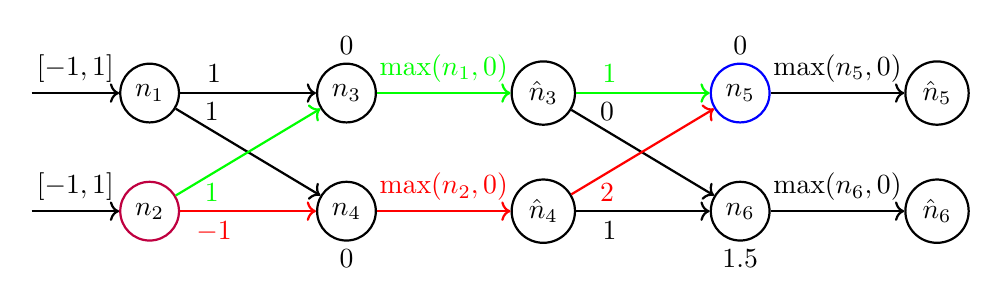
\begin{tikzpicture}
		
		\node[circle, draw= black, thick, minimum width = 20,
		minimum height = 20] (input1) {$n_1$};
		
		\node[circle, draw= purple, thick, minimum width = 20,
		minimum height = 20] (input2) at ($(input1) + (0,-1.5)$) {$n_2$};
		
		
		% Hidden layers
		
		\node (hidden10) at ($(input1) + (2.5,0.6)$) {$0$};
		
		\node (hidden20) at ($(input1) + (2.5,-1.5-0.6)$) {$0$};
		
		\node (hidden50) at ($(input1) + (7.5,0.6)$) {$0$};
		
		\node (hidden60) at ($(input1) + (7.5,-1.5-0.6)$) {$1.5$};
		
		
		\node[circle, draw= black, thick, minimum width = 20,
		minimum height = 20] (hidden1) at ($(input1) + (2.5,0)$) {$n_3$};
		\node[circle, draw= black, thick] (hidden2) at ($(input1) + (2.5,-1.5)$) {$n_4$};
		
		\node[circle, draw= black, thick, minimum width = 20,
		minimum height = 20] (hidden3) at ($(input1) + (5,0)$){$\hat{n}_3$};
		\node[circle, draw= black, thick] (hidden4) at ($(input1) + (5,-1.5)$) {$\hat{n}_4$};
		
		
		\node[circle, draw= blue, thick, minimum width = 20,
		minimum height = 20] (hidden5) at ($(input1) + (7.5,0)$){$n_5$};
		\node[circle, draw= black, thick] (hidden6) at ($(input1) + (7.5,-1.5)$) {$n_6$};
		
		
		
		
		% Output layer
		\node[circle, draw= black, thick, minimum width = 20,
		minimum height = 20] (output1) at ($(input1) + (10,0)$){$\hat{n}_5$};
		
		\node[circle, draw= black, thick, minimum width = 20,
		minimum height = 20] (output2) at ($(input1) + (10,-1.5)$){$\hat{n}_{6}$};
		
		
		% Connections
		
		\draw[->,thick] ($(input1) + (-1.5,0)$) -- (input1) node[midway, above] {$[-1,1]$};
		
		\draw[->,thick] ($(input1) + (-1.5,-1.5)$) -- (input2) node[midway, above] {$[-1,1]$};
		
		
		
		\draw[->,thick] (input1) -- (hidden1) node[near start, above] {$1$};
		\draw[->,thick] (input1) -- (hidden2)node[near start, above] {$1$};
		
		\draw[->,color=green, thick] (input2) -- (hidden1) node[near start, below] {$1$};
		\draw[->,color=red, thick] (input2) -- (hidden2)node[near start, below] {$-1$};
		
		
		
		
		
		\draw[->,color=green, thick] (hidden1) -- (hidden3) node[midway, above] {$\max(n_1,0)$};
		\draw[->,color=red, thick] (hidden2) -- (hidden4) node[midway, above] {$\max(n_2,0)$};
		
		
		
		
		
		\draw[->,color=green, thick] (hidden3) -- (hidden5) node[near start, above] {$1$};			
		\draw[->,thick] (hidden3) -- (hidden6) node[near start, above] {$0$};
		
		\draw[->,color=red, thick] (hidden4) -- (hidden5)node[near start, below] {$2$};
		\draw[->,thick] (hidden4) -- (hidden6)node[near start, below] {$1$};
		
		
		
		
		\draw[->,thick] (hidden5) -- (output1) node[midway, above] {$\max(n_5,0)$};
		\draw[->,thick] (hidden6) -- (output2) node[midway, above] {$\max(n_6,0)$};
		
		
	\end{tikzpicture}
	\caption{A DNN example from \cite{kpoly}: every neuron is separated into 2 nodes, $n$ pre- and $\hat{n}$ post-ReLU activation function. The pair $(n_2 n_3 n_5,n_2 n_4 n_5)$ in green and red is compensating (weights of paths are $1,-2$).}
	\label{fig1}
\end{figure}

The concept of value abstraction involves calculating upper and lower bounds for the values of certain neurons in a Deep Neural Network (DNN) when inputs fall within a specified range. This approach aims to assess the network's robustness without precisely computing the values for every input within that range.

Firstly, it's important to note that weighted sums represent a linear function, which can be explicitly expressed with relative ease. However, the ReLU (Rectified Linear Unit) function presents a challenge in terms of accurate representation. Although ReLU is a relatively straightforward piecewise linear function with two modes (one for $x<0$ and another for $x \geq 0$), it is not linear. The complexity arises when considering the compounded effects of the ReLU function across the various layers of a ReLU DNN. It's worth noting that representing $\ReLU(x)$ precisely is feasible when $x$ is "stable," meaning it's consistently positive or consistently negative, as there's only one linear mode involved in each scenario. Consequently, the primary challenge lies in addressing "unstable" neurons, where the linearity of the function does not hold consistently.


Consider the simpler abstraction, termed ``Box abstraction" \cite{deeppoly}: it inductively computes the bounds for each neuron in the subsequent layer independently. This is achieved by considering the weighted sum of the bounds from the previous layer, followed by clipping the lower bound at $\max(0,$ lower bound$)$ to represent the ReLU function, and so forth. For all $i$, define $x_i=\val_{\vx}(n_i)$, where $\vx=(x_1,x_2)$.

Taking the DNN example from Fig \ref{fig1}, assume $x_1,x_2 \in [-1,1]$. This implies that $x_3,x_4 \in [-2,2]$. After applying the ReLU function, $\hat{x}3,\hat{x}4$ are constrained to $[0,2]$, leading to $x_5 \in [0,6]$ and $x_6 \in [0,2]$. The bounds for $n_1, \ldots, n_4$ are exact, meaning for every $\alpha$ within the range, an input $\vy$ can be found such that $\val{\vy}(n_i)=\alpha$. However, this precision is lost from the next layer (beginning with $n_5, n_6$) due to potential dependencies among preceding neurons. For example, $n_3$ only attains the value $2$ when both $x_1$ and $x_2$ are $2$. In this case, $n_4$ would reach a value of $Val{(2,2)}(n_4)=0$. Consequently, it's implausible for $x_5=\Val_{\vx}(n_5)$ to reach $6$, as it would necessitate both $n_3$ and $n_4$ assuming the value $2$.

An extremely efficient algorithm that addresses some issues is "DeepPoly" \cite{deeppoly}, also independently discovered as the "CROWN" algorithm \cite{crown}. Instead of strict bounds, for each neuron $n$ in layer $k$, DeepPoly maintains two affine functions representing the lower and upper bounds of the neuron's value, based on inputs from the previous layer $k-1$. For instance, denote $f_i \leq x_i \leq g_i$ with, for example, $f_{3}(x_3)=f_4(x_4)=0$ and $g_3(x_3) = \frac{x_3+2}{2}$, $g_4(x_4) = \frac{x_4+2}{2}$. This leads to $x_5 \leq g_3(x_3) + 2 g_4(x_4) = \frac{x_3 + 2x_4 + 6}{2} = \frac{3x_1 - x_2 + 6}{2}\leq 5$.

For bounds $[\alpha,\beta]$ on $x_i$, the optimal linear function for the upper bound is $g_i(x_i)= \beta \frac{x_i-\alpha}{\beta-\alpha}$ for ReLU nodes. There are two options for the lower bound: $f^1_i(x_i) = 0$ or $f^2_i(x_i)=x_i$. DeepPoly selects between these based on the values of $\alpha$ and $\beta$ (for unstable neurons): if $|\alpha|\geq |\beta|$, then $f_i=f^1_i$ is chosen, otherwise, for $|\beta|>|\alpha|$, $f_i=f^2_i$ is selected. The variation, {\em $\overline{\mbox{DeepPoly}}$}, consistently chooses $f^1_i$, and never $f^2_i$. Contrary to DeepPoly, {\em $\overline{\mbox{DeepPoly}}$} encompasses the ``Box abstraction." For instance, with bounds $[-0.2,5]$ on $x_i$, it deduces $\ReLU(x_i) \in [0,5]$, whereas  DeepPoly without box abstraction algorithm would conclude $\ReLU(x_i) \in [-0.2,5]$.


\iffalse
\subsection{PRIMA and $\beta$-CROWN}
\fi

\subsection{MILP and LP encodings for DNNs}

At the other end of the spectrum, we find the Mixed Integer Linear Programming (MILP) value abstraction, which is a priori a complete method (albeit much slower than DeepPoly). 
Consider an unstable neuron $n \in[\alpha,\beta]$. The value $x$ of $\ReLU(n)$ can be encoded exactly in an MILP formula with one integer (actually even binary) variable $a$ valued in ${0,1}$, using 4 constraints \cite{MILP}:
\vspace{-0.1cm}
\begin{align*}
	\hat{x} \geq x \quad \wedge \quad \hat{x} \geq 0, \quad \wedge \quad \hat{x} \leq \beta \cdot a \quad \wedge \quad \hat{x} \leq x-\alpha \cdot (1-a)
\end{align*}

It can be shown that for all $x \in [\alpha,\beta] \setminus 0$, there exists a unique solution $(a,\hat{x})$ that meets these constraints, with $\hat{x}=\ReLU(x)$. Here, $a$ is 0 if $x < 0$, 1 if $x>0$, and can be either if $x=0$~\cite{MILP}. This encoding approach can be applied to every (unstable) ReLU node, and optimizing its value can help in certifying a given input. However, for networks with hundreds of nodes or more, the resulting MILP formulation will contain numerous integer variables and generally cannot be solved efficiently.

MILP instances can be linearly relaxed into LP over-abstraction, where variables originally restricted to integers in ${0,1}$ (binary) are relaxed to real numbers in the interval $[0,1]$, while maintaining the same encoding. As solving LP instances is polynomial time, this optimization is significantly more efficient. However, this efficiency comes at the cost of precision, often resulting in less stringent bounds. This approach is termed the {\em LP abstraction}

The following proposition shows that the LP abstraction refines the DeepPoly abstraction. 
The difference between the LP and the DeepPoly abstractions is that LP simultaneous considers the two linear lower bounding functions for the ReLU operation, namely $ReLU(x) \geq 0$ and $ReLU(x) \geq x$, while the DeepPoly abstraction restricts itself to the application of a single one of these linear bounding functions.
 

\begin{proposition}
	\label{LP}
	Given $x \in [\alpha,\beta]$ with $\alpha < 0 < \beta$, the following two systems of constraints 
	1) for LP and 2) for DeepPoly with both lower bounds are equivalent:
	\begin{align}
& \hat{x} \geq x \quad \wedge \quad \hat{x} \geq 0, \quad \wedge \quad \hat{x} \leq \beta \cdot a \quad \wedge \quad \hat{x} \leq x-\alpha \cdot (1-a), \, a \in [0,1]  \label{eq:lp}\\
&\hat{x} \geq x \quad \wedge \quad \hat{x} \geq 0 \quad \wedge \quad \hat{x} \leq \beta \frac{x-\alpha}{\beta-\alpha} \label{eq:deeppoly}
	\end{align} 
\end{proposition}

\begin{proof}
We need to show that the two upper bound constraints in Eq~\ref{eq:lp} is equivalent to the upper bound in Eq~\ref{eq:deeppoly}. To this end, we focus on the upper bound function in the linear variable $a \in  [0,1]$, with $x \in [\alpha,\beta]$ fixed. We have $\hat{x}$ in Eq~\ref{eq:lp} is upper bounded by $max_{a \in [0,1]} (min(\beta \cdot a, x - \alpha (1-a)))$, and this bound can be reached. Furthermore, 
	The function $\min(\beta \cdot a, x - \alpha (1-a))$ attains its maximum when $\beta \cdot a = x - \alpha (1-a)$, leading to the equation $(\beta - \alpha) a = x - \alpha$ and consequently $a = \frac{x - \alpha}{\beta-\alpha}$. This results in an upper bound of $\beta \cdot a = \beta \frac{x - \alpha}{\beta-\alpha}$ \qed
\end{proof}

\subsubsection*{Constraints for $\gamma$}

We could get the following constraints for $\gamma$, using $y_i$ and $\hat{y}_i$ to denote the $x_i-x_i'$ and $\hat{x}_i-\hat{x}_i'$:\begin{align*}
	\hat{y}_i \leq a \gamma_i \hspace*{2ex} &\wedge \hspace*{2ex}\hat{y} \geq y_i - a \gamma_i\\
	\hat{y}_i \geq (a-1) \gamma_i  \hspace*{2ex} &\wedge \hspace*{2ex} \hat{y} \leq y_i + (1-a) \gamma_i,
\end{align*} where $a$ is a binary variable, $\gamma_i$ is the upper bound of $x_i-\hat{x}_i$.

\hspace*{-20ex}

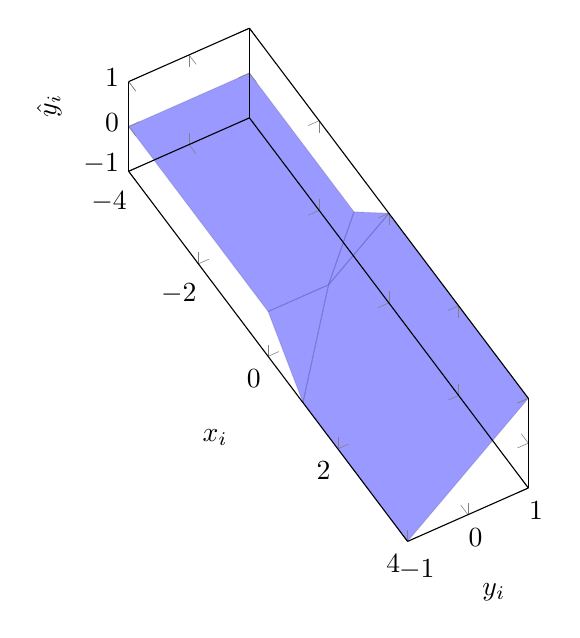
\begin{tikzpicture}
	\begin{axis}[	axis on top, xlabel = \(x_i\),
		ylabel = {\(y_i\)}, zlabel = \(\hat{y}_i\),
				set layers=default,
	xmax = 4, xmin = -4,
ymax = 1, ymin = -1,		
zmax = 1, zmin = -1,
				unit vector ratio=1 1 1, scale=1.5,
				view={60}{50},
				]
		\addplot3[fill=blue,opacity=0.1, fill opacity=0.4] 
		coordinates {
	 (0,0,0) (-1,1,0) (-4,1,0) (-4,-1,0) (0,-1,0) (0,0,0)
		};
		
		\addplot3[fill=blue,opacity=0.1, fill opacity=0.4	] 
		coordinates { (0,0,0) (0,1,1) (4, 1, 1) (4, -1, -1) (1,-1,-1) (0,0,0)
		};
		
		\addplot3[fill=blue,opacity=0.1, fill opacity=0.4	] 
		coordinates { (0,0,0)  (-1,1,0) (0,1,1) (0,0,0)
		};
		
			\addplot3[fill=blue,opacity=0.1, fill opacity=0.4	] 
		coordinates { (0,0,0)  (0,-1,0) (1,-1,-1) (0,0,0)
		};
		
	\end{axis}
\end{tikzpicture}


\hspace*{-20ex}

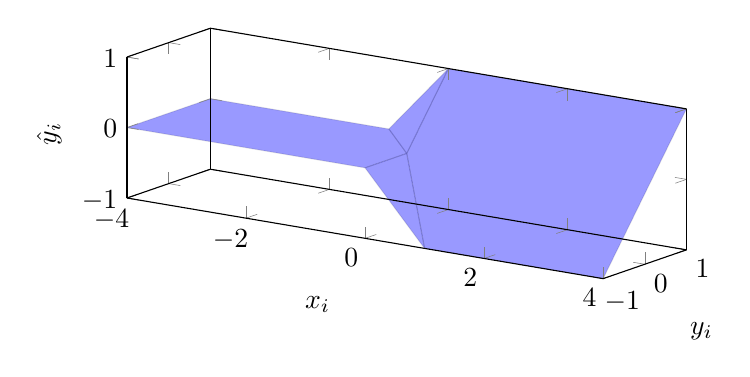
\begin{tikzpicture}
	\begin{axis}[	axis on top, xlabel = \(x_i\),
		ylabel = {\(y_i\)}, zlabel = \(\hat{y}_i\),
		set layers=default,
				xmax = 4, xmin = -4,
		ymax = 1, ymin = -1,		
				zmax = 1, zmin = -1,
		unit vector ratio=1 1 1, scale=1.5,
		view={35}{14},
		]
		\addplot3[ fill=blue,opacity=0.1, fill opacity=0.4] 
		coordinates {
			(0,0,0) (-1,1,0) (-4,1,0) (-4,-1,0) (0,-1,0) (0,0,0)
		};
		
		\addplot3[	fill=blue,opacity=0.1, fill opacity=0.4] 
		coordinates { (0,0,0) (0,1,1) (4, 1, 1) (4, -1, -1) (1,-1,-1) (0,0,0)
		};
		
		\addplot3[	fill=blue,opacity=0.1, fill opacity=0.4	] 
		coordinates { (0,0,0)  (-1,1,0) (0,1,1) (0,0,0)
		};
		
		\addplot3[	fill=blue,opacity=0.1, fill opacity=0.4	] 
		coordinates { (0,0,0)  (0,-1,0) (1,-1,-1) (0,0,0)
		};
		
	\end{axis}
\end{tikzpicture}


%\begin{tikzpicture}[
%	declare function={
%		f(\x,\y)=max((\x+\y),0)-max(\x,0);
%	}]
%	\begin{axis}[axis lines=center,
%		axis on top,
%		set layers=default,
%		xrange=-3:3,
%		yrange=-2:2,
%		unit vector ratio=1 1 1,% <- HERE (taken from Phelype Oleinik's deleted answer)
%		scale=3 %<- added to compensate for the downscaling
%		% resulting from unit vector ratio=1 1 1
%		]
%		\addplot3[
%		domain=-3:3,
%		domain y=-1:1, surf,
%		samples=40,
%		samples y=40,
%		] {f(\x,\y)};
%	\end{axis}
%\end{tikzpicture}


\section{Solution-Aware Scoring.}

\label{sec4}

In this section, we propose {\em Solution-Aware Scoring} (SAS),
to evaluate accurately how opening a ReLU impacts the accuracy.
To do so, SAS considers explicitly a solution to a unique LP call, which is reasonably fast to obtain as there is no binary variables (polynomial time). 
%To compute $\Delta(z)$, intermediate $\Delta(b),\Delta(\hat{b})$ are computed inductively.
%Indeed, it is not rare that $z$ is sensitive to ReLU node $n$, and yet $\LP(n)$ already provides an accurate approximation of $\ReLU(n)$.
%In this case, usual heuristics would open $n$, while it would only improve the value of $z$ in a limited way.
Assume that we want to compute an upper bound for neuron $z$ on layer $\ell_z$.
We write $n < z$ if neuron $n$ is on a layer before $\ell_z$, and $n \leq z$ if $n< z$ or $n=z$. We denote ($\Sol\_\max_X^z(n))_{n \leq z}$ a solution of $\mathcal{M}_X$ maximizing $z$: $\Sol\_\max_X^z(z)$ is the maximum of $z$ under $\mathcal{M}_X$.

Consider $(sol(n))_{n \leq z} = (\Sol\_\max_\emptyset^z(n))_{n \leq z}$, a solution maximizing the value for $z$ when all ReLU use the LP relaxation.
%(this can be obtained very efficiently by {\em one} call to an LP solver).
Function
$\Improve\_\max^z(n)=$ $\sol(z) - \Sol\_\max_{\{n\}}^z(z)$, 
accurately represents how much opening neuron $n < z$ reduces the maximum computed for $z$
compared with using only LP. 
We have $\Improve\_\max^z(n)\geq 0$ as $\Sol\_\max_{\{n\}}^z$ fulfills all the constraints of 
$\mathcal{M}_\emptyset$, so $\Sol\_\max_{\{n\}}^z(z) \leq \sol(z)$.
%Similarly, we define ($\Sol\_\min_\emptyset^z(n))_{n \leq z}$ and 
%$\Improve\_\min^z(n)$. 
Computing exactly $\Improve\_\max^z(n)$ would need a MILP call on $\mathcal{M}_{\{n\}}$ for every neuron $n \leq z$, which would be very time consuming. Instead, the SAS function uses a (single) LP call to compute $(sol(n))_{n \leq z}$, with negligible runtime wrt the forthcoming  $\MILP_X$ call, and yet accurately approximates $\Improve\_\max^z(n)$ 
(Fig. \ref{fig_table3}).


\iffalse
That's why as far as we know, in competing heuristics to rank important nodes (e.g. \cite{BaB,huang2017safety,ferrari2022complete}), no call to solvers are made.
%Instead, we focus on the following $\Utility\_\max\nolimits^z(n)$ function upper bounding $\Improve\_\max^z(n)$. 
\fi





%\subsubsection*{Observation}

%The key of our formula is based on the following observation:



%Our observation (by experiments) is that \begin{align}
%	I_X \approx \sum_{b\in X} I_b.
%\end{align} Especially, if all neurons in $X$ are from one layer before $a$, then in %experiments, we observe that 

\iffalse
\begin{align*}
	|(I_X - \sum_{b\in X} I_b)/I_X| < 1\%. \ (\text{in experiments})
\end{align*} Even $X$ contains neurons from 3 layers before the target layer, in experiments, $I_X$ is still close to $\sum_{b\in X} I_b$.

Therefore, based on this observation, the question to choose $X$ is converted to compute $I_b$ for neurons $b$ in layers before the target layer. Our formula is to estimate the improvement of different individual neurons in different layers. For different layers, the formula will be different.  However, neither the observation in this subsection nor the formula in the next subsection has solid theoretical proof to show that they are very accurate. They are all based on experiments. 


In our algorithm, we will open neurons at most 3 layer3 before the target layer. So the formula will consists of three parts.


\subsubsection*{Compute the improvement of a single neuron}

\subsection*{One Layer before $z$}

\fi

%For all neurons $n$, let $\sol(n)=$$\Sol\_\max_\emptyset^z(n)$ be the value of neuron $a$
%in the solution of the LP instance $\Sol\_\max_\emptyset^z$ to maximize $z$.
%For one layer before the target layer, the formula is simple and most accurate. 
%To estimate $\Improve\_\max^z(a)$, 



%we define $\Utility\_\max^z(a)$, first for neurons $a$ one layer before $z$, by computing by how much the value of $z$ will change if $a$ is opened
%and other values remain the same - in particular, $value(\hat{a})=\ReLU(sol(a))$. We define:
%we first need to run $M^a_{\emptyset}$ to compute the upper bound of $a$  to obtain the solution data. Especially, we will read the values of $b$, before $\ReLU$ function and after $\ReLU$ function.

For a neuron $b$ on the layer before layer $\ell_z$, we define:


\vspace{-0.4cm}
	$$\Utility\_\max\nolimits^z(b) = W_{bz} \times (\sol(\hat{b})- \ReLU(\sol(b)))$$
\vspace{-0.4cm}
	
	%In particular, if $\sol(\hat{a})=\ReLU(\sol(a))$, then we will have 
	%\begin{align*}
%		Utility^z(a) = 0.
%	\end{align*}


\noindent {\em Comparison:} consider $b$ with $W_{bz}<0$: 
to maximize $z$, the value of $\sol(\hat{b})$ is minimized by LP, 
ie $\sol(\hat{b})=\ReLU(\sol(b))$ thanks to Proposition~\ref{LP}. 
Thus, we have $\Utility\_\max^z(b)=0=\Improve_{max}^z(b)$.
Notice that the original scoring function $|W_{bz}|(\UB(b)-\LB(b))$ \cite{DivideAndSlide}  would be possibly very large in this case. However, {\sf GS} scoring functions from BaB-SR and FSB would also accurately compute  $s_{FSB}(b)=s_{SR}=0$.
Notice that $\Utility$ does not need to consider bias explicitly, unlike $s_{FSB},s_{SR}$,
as they are already accounted for in the solution considered. 

\medskip

Consider a neuron $a$ two layers before $\ell_z$, 
$b$ denoting neurons in the layer $\ell$ just before $\ell_z$.
Recall the rate $r(b)=\frac{\max(0,\UB(b))}{\max(0,\UB(b))-\min(0,\LB(b))} \in [0,1]$.
We define:


\begin{flalign*}
	\Delta(\hat{a}) &= \ReLU(\sol(a))-\sol(\hat{a})&&\\
	\forall b \in \ell, \Delta(b) &= W_{ab}\Delta(\hat{a})&&\\	
\end{flalign*}

\vspace{-1.2cm}

\begin{subnumcases}{\forall b \in \ell, \Delta(\hat{b}) =}
		r(b)\Delta(b), & for $W_{bz} > 0$ \\
		\max(\Delta(b),-\sol(b)), & for $W_{bz} < 0$ and $\sol(b)\geq0$\\
		\max(0,\Delta(b)+\sol(b)), & for $W_{bz} < 0$ and $\sol(b)<0$ \quad \, \quad \, \quad		 
\end{subnumcases}

\begin{flalign*}
	\Utility\_\max\nolimits^z(a) &= \Delta(z) = -\sum_{b \in \ell} W_{bz} \Delta(\hat{b})&&
\end{flalign*}





\begin{figure}[t!]
	\begin{centering}
	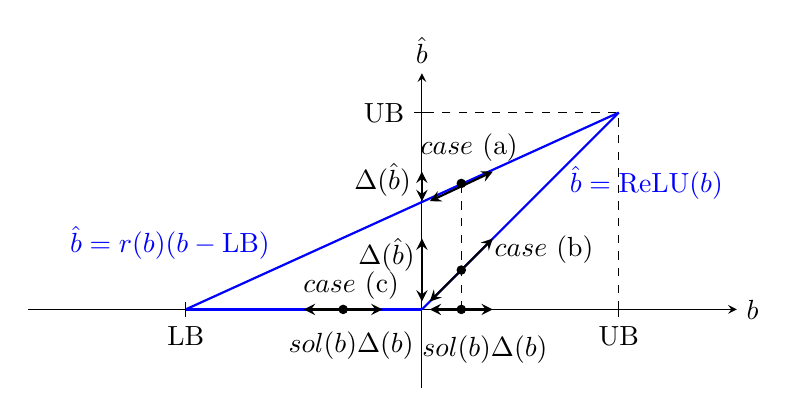
\begin{tikzpicture}[scale=1, >=stealth]
		
		% Draw axes
		\draw[->] (-5,0) -- (4,0) node[right] {$b$};
		\draw[->] (0,-1) -- (0,3) node[above] {$\hat{b}$};
		
		% Draw ReLU function
		\draw[line width=0.4mm, blue] (-3,0) -- (0,0);
		\draw[thick, blue] (0,0) -- (2.5,2.5) node[below, shift={(0.35,-0.55)}] {$\hat{b} = \ReLU(b)$};
		\draw[thick, blue] (-3,0) -- (2.5,2.5) node[above, shift={(-5.7,-2)}] {$\hat{b} = r(b) (b-\LB)$};
		
		% Add labels
		\draw[dashed] (2.5,0) -- (2.5,2.5) -- (0,2.5); % Optional grid
		\node[below left] at (0,0) {};
		
		% Add tick marks
		
		\foreach \x in {2.5}
		\draw[shift={(\x,0)}] (0,0.1) -- (0,-0.1) node[below] {$\UB$};
		\foreach \x in {-3}
		\draw[shift={(\x,0)}] (0,0.1) -- (0,-0.1) node[below] {$\LB$};
		
		\foreach \y in {2.5}
		\draw[shift={(0,\y)}] (0.1,0) -- (-0.1,0) node[left] {$\UB$};
		
		\draw[<->, thick] (0.1, 0.1) -- (0.9, 0.9) node[above,shift={(0.65,-0.45)}] {$case$ (b)}
		node[below,shift={(-0.1,-1.10)}] {$sol(b)\Delta(b)$}
		node[above,shift={(-1.35,-0.55)}] {$\Delta(\hat{b})$};
		\filldraw[black] (0.5, 0.5) circle (1.5pt);
		\filldraw[black] (0.5, 0) circle (1.5pt);
		\draw[<->, thick] (0.1, 0) -- (0.9, 0);
		\draw[dashed] (0.5,0) -- (0.5,1.6); % Optional grid
		
		
		\draw[<->, thick] (-0.5, 0) -- (-1.5, 0) node[above,shift={(0.6,0)}] {$case$ (c)}
		node[below,shift={(0.6,-0.15)}] {$sol(b)\Delta(b)$};
		\filldraw[black] (-1, 0) circle (1.5pt);
		
		
		\draw[<->, thick] (0.1, 1.375) -- (0.9, 1.75) node[above,shift={(-0.3,0)}] {$case$ (a)}
		node[above,shift={(-1.4,-0.45)}] {$\Delta(\hat{b})$};
		\filldraw[black] (0.5, 1.6) circle (1.5pt);
		
		\draw[<->, thick] (0, 0.1) -- (0, 0.9);
		
		\draw[<->, thick] (0, 1.375) -- (0, 1.75);

	\end{tikzpicture}
	\caption{Different cases for $\ReLU(b)$
	 \vspace{-0.3cm}}
	\label{node:b}
\end{centering}
\end{figure}

%\begin{tikzpicture}[scale=1, >=stealth]
%	
%	% Draw axes
%	\draw[->] (-5,0) -- (4,0) node[right] {$x$};
%	\draw[->] (0,-1) -- (0,3) node[above] {$y$};
%	
%	% Draw ReLU function
%	\draw[line width=0.4mm, blue] (-3,0) -- (0,0);
%	\draw[thick, blue] (0,0) -- (2.5,2.5) node[below, shift={(0.5,-0.4)}] {$y = \ReLU(x)$};
%	\draw[thick, blue] (-3,0) -- (2.5,2.5) node[above, shift={(-0.5,0.4)}] {$y = \frac{\UB}{\UB-\LB} x-\frac{\UB\LB}{\UB-\LB}$};
%	
%%	% Add labels
%%	\draw[dashed] (2,0) -- (2,2) -- (0,2); % Optional grid
%%	\node[below left] at (0,0) {$0$};
%%	
%%	% Add tick marks
%%	\foreach \x in {1,2}
%%	\draw[shift={(\x,0)}] (0,0.1) -- (0,-0.1) node[below] {\x};
%%	\foreach \y in {1,2}
%%	\draw[shift={(0,\y)}] (0.1,0) -- (-0.1,0) node[left] {\y};
%	
%\end{tikzpicture}

%We will show with a more general definition that $0 \leq \Improve\_\max^z(a) \leq \Utility\_\max^z(a)$ in Prop.~\ref{prop2}. 

%Informally, $\Delta(\hat{a}), \Delta(b), \Delta(\hat{b})$ approximate the improvement on the accuracy of $\hat{a}, b, \hat{b}$ when computing $\ReLU(a)$ using the exact MILP encoding instead of LP. 

{\color{red}
\noindent {\em Comparison:} First, the original \cite{DivideAndSlide} does not propose a formula for node $a$ two layers before $z$. 
Consider again the running example of Fig. \ref{img:FSB_example}. 
In the case $c\cdot d<0$, we have $\Utility\_\max\nolimits^z(a)=\Improve_{max}^z(b)=s_{FSB}(a)=s_{SR}(a)=0$, as $\Delta(\hat{a})=0$. In the case $c>0,d>0$, 
$\Delta(\hat{a}) = \ReLU(\sol(a))-\sol(\hat{a})$ is precise,
whereas the corresponding $\Delta_{FSB}(\hat{a}) = \LB(a) r(a)$ is only an upperbound.
The last case $c<0,d<0$ is the most extreme: 
$\Delta(\hat{b})$ adapts to the case (b),(c) in Fig. \ref{node:b} leveraging the value $\sol(b)$, which yields very different values, whereas the corresponding $\Delta_{FSB}(\hat{b})$
is always $r(b) \Delta_{FSB}(b)$. For $sol(b)<<0$, we will have 
$\Delta(\hat{b})=0<\Delta_{FSB}(\hat{b})$.
For $sol(b)>>0$, we will have 
$\Delta(\hat{b})=\Delta(b) > \frac{1}{2}\Delta_{FSB}(\hat{b})$ 
as $r(b)=\frac{1}{2}$. We can show that $\Utility$ is a safe overapproximation of 
$\Improve\_\max^z(a)$, which does not hold for $s_{FSB},s_{SR}$ (because of the case $sol(b)>>0$):
}

\begin{proposition}
	\label{prop2}
		$0 \leq \Improve\_\max^z(a) \leq \Utility\_\max^z(a)$. 
\end{proposition}


In particular, for all nodes $a$ with $\Utility\_\max\nolimits^z(a)=0$, 
we are sure that this node is not having any impact on $\Sol\_\max_{\{a\}}^z(z)$. 
%This is one striking difference (but not the only one) with choosing utility based on 
%$|W_{az}|$ \cite{DivideAndSlide}.

	
%	
%	Similarly, let $\sol(b)$ be the value of $b$ in the LP solution of lower bound of $a$, and $\sol(\hat{b})$ be the value of $\hat{b}$. Then the formula to estimate improvement of lower bound of $b$ is: \begin{align*}
%		Improve\_min^z(b) \approx -W_{ba}(\sol(\hat{b})-\ReLU(\sol(b))).
%	\end{align*}
	
%To explain the formula, we use upper bound and the case that $W_{ba} > 0$ as an example. To compute the upper bound of $a$, $\hat{b}$ should be as large as possible. In the LP model, for fixed $\sol(b)$, the upper bound of $\hat{b}$ may be larger than $\ReLU(\sol(b))$. This is because in LP model, the upper bound of $\sol(\hat{b})$ is decided by the linear approximation rather than $\ReLU$ function. So, when neuron $b$ is open, if $\sol(b)$ do not change, then the upper bound of $a$ will be improved because the value of $\sol(\hat{b})$ will be lower to $\ReLU(\sol(b))$.
% 			
%Of course changing other variables may also effect the upper bound, but our experiments show that, the change from $\sol(\hat{b})$ to $\ReLU(\sol(b))$ is the major part of improvement. 


 



	
	\begin{proof}
    Consider $\sol'(n)_{n \leq z}$ with
	$\sol'(n)=\sol(n)$ for all $n \notin \{z,\hat{a}\} \cup \{b,\hat{b} \mid b \in \ell\}$. In particular,  $\sol'(a) = \sol(a)$.
	Now, define $\sol'(\hat{a}) = \ReLU(\sol(a))$. 
	That is, $\sol'(\hat{a})$ is the correct value for $\hat{a}$, obtained if we open neuron $a$, compared to the LP abstraction for $\sol(\hat{a})$.
	We define $\sol'(b)=\sol(b)+\Delta(b)$ and 
	$\sol'(\hat{b})=\sol(\hat{b}) + \Delta(\hat{b})$.
	Last, $\sol'(z)=\sol(z) + \sum_{b \in \ell} W_{bz} \Delta(\hat{b})$.
	We will show:
	\begin{equation}
		\label{eq12}
		(\sol'(n))_{n \leq z} \text{ satisfies the constraints in } \mathcal{M}_{\{a\}}
	\end{equation} 
	This suffices to conclude: as
	$\sol'(z)$ is a solution of $\mathcal{M}_{\{a\}}$, it is smaller or equal to the maximal solution: $\sol'(z) \leq$ $\Sol\_\max_{\{a\}}^z(z)$. That is, 
	$\sol(z)-\sol'(z) \geq \sol(z) -$ $\Sol\_\max_{\{a\}}^z(z)$, i.e. 
	$ \Utility\_\max^z(a) \geq \Improve\_\max^z(a)$.
	In particular, we have that $\Utility\_\max^z(a) \geq 0$, which was not obvious from the definition.	

Finally, we show (\ref{eq12}). First, opening $a$ changes the value of $\hat{a}$ from
	$\sol(\hat{a})$ to $\ReLU(\sol(a)) = sol(\hat{a}) + \Delta(a)$, 
	and from $sol(b)$ to $sol(b) + \Delta(b)$.
	The case of $\Delta(\hat{b})$ is the most interesting:
	If (a) $W_{bz}>0$, to maximize $z$, the LP solver sets $\sol(\hat{b})$ to the maximal possible value, which is 
	$r(b) \sol(b)+$ Cst according to Proposition \ref{LP}.
Changing $b$ by $\Delta(b)$ thus results in changing $\sol(\hat{b})$ by 
$r(b) \Delta(b)$.
If $W_{bz}\leq0$, then the LP solver sets $\sol(\hat{b})$ to the lowest possible value to maximize $z$, which happens to be $\ReLU(b)$ according to Proposition \ref{LP}.
If (b) $\sol(b) > 0$, then 
$\sol(\hat{b})=\ReLU(\sol(b))=\sol(b)$, and the change to $\hat{b}$ will be 
the full $\Delta(b)$, unless $\Delta(b) < -\sol(b) < 0$ in which case it is 
$-\sol(b)$.
If (c) $\sol(b) < 0$, then we have $\sol(\hat{b})=\ReLU(b)=0$ and opening $a$ moves away 
from 0 only if $\sol(b)+\Delta(b)>0$. 
\qed
\end{proof}


\iffalse

	If we open $a$ without changing its value $\sol(a)$, then the change $\Delta(\hat{a})$ in the weight of $\hat{a}$ is 
$\Delta(\hat{a})=\ReLU(\sol(a)) - \sol(\hat{a}) \leq 0$ as above. Its impact on $z$ is no more direct with $W_{az}$, but it is through $\ell$. 
We let $\Delta(b) = W_{ab}\Delta(\hat{a})$ for all $b \in \ell$.
Based on Proposition \ref{LP}, we can evaluate the impact 
$\Delta(\hat{b})$ of opening $a$ on the value of each $\hat{b}$, by using the upper and lower bound $\UB(b),\LB(b)$:

	\begin{align*}
		&\Delta(\hat{b}) =
		\begin{cases}
			\frac{\UB(b)}{\UB(b)-\LB(b)}\Delta(b),  &\text{if }W_{bz} > 0\\
			\max(\Delta(b),-\sol(b)),  &\text{if }  W_{bz} < 0 \text{ and } \sol(b)\geq0\\
			\max(\Delta(b)+\sol(b),0),  &\text{if }  W_{bz} < 0 \text{ and } \sol(b)<0		 
		\end{cases}
		\end{align*}


Indeed, if $W_{bz}>0$, then according to Proposition \ref{LP}, the LP solver
sets $\sol(\hat{b}) = \sol(b) \frac{\UB(b)}{\UB(b)-\LB(b)} +$ Cst to maximize $z$.
Changing $b$ by $\Delta(b)$ thus results in changing $\sol(\hat{b})$ by 
$\frac{\UB(b)}{\UB(b)-\LB(b)}\Delta(b)$.
If $W_{bz}\leq0$, then the LP solver sets $\sol(\hat{b})$ to the lowest possible value to maximize $z$, which happens to be $\ReLU(b)$ according to Proposition \ref{LP}.
If $\sol(b) < 0$, then we have $\sol(\hat{b})=\ReLU(b)=0$ and opening $a$ change the 0 value only if $\sol(b)+\Delta(b)>0$. If $\sol(b) > 0$, then 
$\sol(\hat{b})=\ReLU(\sol(b))=\sol(b)$, and the change to $\hat{b}$ will be 
the full $\Delta(b)$, unless $\Delta(b) < -\sol(b) < 0$ in which case it is 
$-\sol(b)$. We then set:

%We then define 
%\begin{align*}
%	Utility\_max^z(a) = (\sol(\hat{a})-\ReLU(\sol(a)))\sum_b k(b).
%\end{align*}

$$ \Utility\_\max\nolimits^z(a) = -\sum_{b \in \ell} W_{bz} \Delta(\hat{b})$$
\fi

%We proceed inductively to define $\Utility\_\max^z(a)$ for deeper neurons $a$.

\iffalse
While $\Utility$ is a priori a more accurate way to select neurons to open in partial MILP (that will be verified in Fig. \ref{fig_table3}), global scoring functions have two advantages: first, they are faster to compute (a unique backpropagation is sufficient, while SAS needs one LP call to recover the solution, plus a forward propagation for each node $a$). This is not an issue for selecting nodes for partial MILP, as there is a single selection step. This would be potentially problematic for choosing branching nodes in BaB, at each branch. A trade off could be to precompute FSB and only on the most promising nodes run $\Utility$. The second shortcoming is the other side of the coin to consider improvement local to a solution: in the case of branching, one of the branch imposes to be far from the solution and $\Utility$ is not accurate on that branch, while global scoring is as (in)accurate for both branches. We will verify that using GS for ordering nodes after the SAS selection is actually more efficient, for this very reason.
\fi

%\textcolor{red}{$s_{FSB}$ *is* in Figure 5, under label “GS” (global-scoring). $s_{SR}$ is very slightly worst, reason why we did not report it.}

\iffalse
We use the following formula for general cases, i.e. possibly more than 3 layers. We use $a$ to denote the source node, and use $b,c$ to denote that $b$ is in one layer before $c$. 

\begin{align*}
	\Delta(\hat{a}) &= \ReLU(\sol(a))-\sol(\hat{a})\\
	\Delta_0(b) &= \sum_{b} W_{bc}\Delta(\hat{b})\\
		\Delta(c) &= \min(\max((\sol(c)+\Delta_0(c),\LB(c))),\UB(c))-\sol(c)\\
		\Delta(\hat{c}) &=
		\begin{cases}
		\Delta(c)\frac{\LB(c) - \sol(\hat{c})}{\LB(c) - \sol(c)},  &\text{if } \LB(c)< \sol(c) < 0\\
		\Delta(c)\frac{\UB(c) - \sol(\hat{c})}{\UB(c) - \sol(c)},  &\text{if }  0< \sol(c) < \UB(c)\\
			\Delta(c),  &\text{else } 	 
		\end{cases}
\end{align*}


\subsubsection*{Three Layer before  $z$} 

Suppose $a$ is a neuron in three layers before $z$, we use $b$ to denote neurons in two layer before $z$ and $c$ to denote neurons in one layer before $z$ and. 

This formula is based on previous subsection but more complex. In some network, running this formula may cost too much time. 

The key problem is how to compute the coefficient $k$ for neurons in two layers before the target layer. To do this, we may use the values in the solution of LP model as follows:

\begin{definition}\label{3layer}
Let $\UB$ and $\LB$ denote the precomputed upper bounds and lower bounds used in building MILP models. We define the following function $h$ for all neurons $b$ in two layers before the target neuron $z$ as follows:
	\begin{align}
		&v_0 = \sol(\hat{b}), v_1 = \ReLU(\sol(b)), v_2 = \frac{\UB(b)\sol(b)-\UB(b)\LB(b)}{\UB(b)-\LB(b)}\\
		&h(b) =
		\begin{cases}
			\frac{v_0-v_1}{v_2-v_1}, & \text{if } v_2-v_1 > 0\\
			0.5, & \text{otherwise.}
		\end{cases}
	\end{align} 
\end{definition} 

\begin{definition}
	Continue the assumption in Definition \ref{3layer}. We define function $D$ layer by layer.
	
	First, $\Delta(a) = \ReLU(\sol(a))-\sol(\hat{a})$.
	
To compute $\Delta(b)$ for neurons $b$ in two layer before $z$, we define \begin{align}
	&u_0 = \max(\LB(b),\min(\UB(b),  \sol(b)+\Delta(a)W_{ab}))\\
	&u_1 = \begin{cases}
		\ReLU(u_0)+h(b)(\frac{\UB(c)u_0-\UB(b)\LB(b)}{\UB(b)-\LB(b)}-\ReLU(u_0)), & \text{if }\LB(b) < 0\\
	u_0, & \text{if }  \LB(b) \geq 0
	\end{cases}\\
	&\Delta(b) = u_1-\sol(\hat{b})
\end{align}
	
	To compute $\Delta(c)$ for neurons $c$ in one layer before $z$, we define 
	\begin{align}
		&w_0 = \sum_b \Delta(b)W_{bc}\\
		&w_1 = \min(\UB(c),\sol(c)+w_0)\\		
		&\Delta(c) =
		\begin{cases}
			w_1-\sol({c}), & \text{if }W_{cz} > 0 \text{ and } \LB(c)\geq 0\\
		k(c)(w_1-\sol({c})), & \text{if }W_{cz} > 0 \text{ and } \LB(c)< 0\\
		\ReLU(w_1)-\sol(\hat{c})	, & \text{if }  W_{cz} < 0
		\end{cases}\\
		&\Delta(z) = \sum_c \Delta(c)W_{cz}\\
		&\Utility\_\max^z(a) = -\Delta(z)
	\end{align}
\end{definition}
		
\fi




	\section{Experimental Evaluation}
	
	We implemented our code in Python 3.8.
	Gurobi 9.52 was used for solving the MILP problems. We conducted our evaluation on an AMD Threadripper 7970X ($32$ cores$@4.0$GHz) with 256 GB of main memory and 2 NVIDIA RTX 4090. 
	
	We consider 4 pretrained DNNs on 3 different datasets (MNIST, Fashion MNIST and CIFAR10). Namely,  MNIST-FC, a fully connected DNN available at 
	\url{https://github.com/eth-sri/eran} ("5x100"). We also considered 3 convolutional DNNs: MNIST-Conv, FMNIST-Conv, and CIFAR10-Conv, 
	from \cite{vhagar} ("conv1"). We will also consider 3 PCA-DNNs, as detailled in Section~\ref{s62}
	%The pipe considers a conjunction of $L_1 \leq 3.9$ and $L_\infty \leq .02$ perturbations, physically pertinent dimensions, and maximizes the sum of the difference in output of 10 selected points in the mesh between input and its deformation.

\iffalse	
For each benchmark, we report three values: the bound obtained (lower value is better), the solution obtained (distance to the bound depicts how close the model has converged), and worst-case (higher is better), that is the value reached when considering the solution as input to the DNN. For a fully accurate model ("2v" or classical and all variables binary), the worst-case will equal the solution, otherwise, it will be smaller due to abstraction.
\fi

%\subsection{Classical vs our "2v" model vs ITNE}
%
%
%\begin{table}[b!]
%	\centering
%	\begin{tabular}{||l|c|c|c||}\hline\hline
%		model, nbr binary var &        Bound $\downarrow$ &  Sol. &      Worst-Case $\uparrow$ \\\hline \hline
%	Classical, $100$ &    $.320$ &  $.320$ & $.017$ 
%    \\\hline
%	ITNE, $100$ &    $.042$ &  $.037$ & $.022$
%	\\ \hline
%    2v model, $100$ &    {\bf .040} &  $.037$ &  $.018$ 
%    \\\hline \hline
%     2v model New, $100$ &    {\bf .039} &  $.029$ &  $.020$ 
%    \\\hline \hline
%    Classical, $200$ &  .186  &  $.022$ & $.022$ 
%    \\\hline
%	ITNE, $200$ &    $.045$ &  $.023$ & .023
%    \\\hline
%	2v model, $200$&     {\bf .042} &  $.023$ &   .023 
%    \\\hline \hline
%	\end{tabular}
%	\caption{Comparison of the classical encoding, ITNE and our "2v" model on the pipe system with a fixed timeout of 1000s, with either $100$, 
%    or the full $200$ binary variables.}
%    \label{table.classical}
%\end{table}
%
%We start by evaluating how accurate the 2v model is vs the classical encoding vs the interleaving twin-network encoding (ITNE) from \cite{lipshitz,ITNE}, that we reimplement by considering the classical encoding plus the explicit constraints $\frac{x_i-x_i' - \gamma}{2} \leq \hat{x}_i-\hat{x}_i' \leq \frac{x_i-x_i' + \gamma}{2}$, corresponding to Eq. (3) of \cite{ITNE} (and also to our (\ref{eq.lpr})). We compare when half the ReLUs are approximated with the LP relaxation, and when all the ReLUs are encoded exactly. We consider the pipe surrogate as it is easier to verify, and set the time-out at 1000s for all models.
%
%
%Table \ref{table.classical}, $100$, confirms that the LP relaxation of the classical model is extremely poor, with bounds $8$ times worse than using our "2v" model, when 50 variables use LP relaxation. Adding explicitly LP relaxation constraints of Eq. (3) from \cite{ITNE} recovers most but not all the bound of the "2v" model.
%
%Further, even using a fully accurate model with all $100$ variables encoded as binary variables, the "2v" model produces bounds $>4$ times better than the classical model, due to the internal Branch and Bound process to compute bounds, which uses linear relaxation. Again, 
%Eq. (3) from \cite{ITNE} recovers most but not all the accuracy of the "2v" model.
%Overall, the "2v" model produces better bounds, even with short time-outs, despite its higher complexity.






\subsection{Comparison for global robustness with VHAGaR and ITNE}

We use VHAGaR benchmarks to be able to compare: 
bound $\alpha$, perturbation $L_\infty=0.05$, VHAGaR convolutional DNNs, for which the VHAGaR reduction rules of binary variables are implemented. We tested with 1000s and 14400s (4h) timeout. We report the upper bound $\bar{\alpha}$ each MILP model find. For each DNN, we report the best lower bound $\underline{\alpha}$ among the MILP models, and report the gap between $\bar{\alpha}$ and  $\underline{\alpha}$ as $\%$ of increase over $\underline{\alpha}$. We report results in Table \ref{table.classical}. Recall most robustness tools, e.g. $\alpha,\beta$-Crown, can only handle {\em local} robustness and cannot be tested.

\iffalse

\begin{table}[h!]
	\centering
	\begin{tabular}{||c||c|c|c|c|c||}\hline\hline
	Benchmark & model & Bound $\downarrow$ &  Sol. &      Worst-Case $\uparrow$ & $\%$ of gap $\downarrow$ \\\hline \hline
	MNIST   & VHAGaR & 20.51 & 9.20 & 9.20 & 118 $\%$
    \\
	M-Conv & ITNE & 12.77 & 9.41 & 9.41 & 35 $\%$
	\\ 
    TO=1000s & {\em Diff} & {\bf 11.59}  & 9.38 & 9.38 & {\bf 23 $\%$}
    \\\hline \hline

	FMNIST & VHAGaR &  $41.52$ & $21.23$ & $21.23$ & 93 $\%$ 
    \\
	F-Conv  & ITNE &  $27.57$ &  $22.12$ & $22.12$ & 24 $\%$
	\\ 
    TO=1000s & {\em Diff} &  {\bf 23.67} &  $22.31$ &  $22.31$ & {\bf 6 $\%$}
    \\\hline 


	FMNIST & VHAGaR &  $37.26$ &  $22.00$ & $22.00$ & 72 $\%$
    \\
	F-Conv  & ITNE &  $24.56$ &  $22.20$ & $22.20$ & 10 $\%$
	\\ 
    TO=14400s & {\em Diff} &    {\bf 22.56} &  $22.32$ &  $22.32$ & {\bf 1 $\%$}
    \\\hline \hline
	
	CIFAR-10  & VHAGaR & does & not & run & -
    \\
	C-Conv  & ITNE & 28.61 & 11.58 & 11.58 & $33\%$
	\\ 
    TO=1000s & {\em Diff} &  25.93  & 14.43 & 14.43 & $24\%$
	\\
	& {\em 2b+1} &  25.31 & 19.77 & - & $23\%$
	\\
	& Best &  {\bf 23.44}  &  &  & {\bf 16} $\%$
    \\\hline
    
	CIFAR-10  & VHAGaR & does & not & run & -
    \\
	C-Conv  & ITNE &  & & &
	\\ 
    TO=14400s & {\em Diff} &  {\bf 20.67}  & 19.03 & 19.03 & {\bf 6} $\%$
	\\
	 & {\em 2b+1} &  {\bf }  &  &  & $\%$
    \\\hline \hline
    

     \end{tabular}
	\caption{Comparison with VHAGaR for $L_\infty=0.05$ perturbation.}
    \label{table.classical}
\end{table}


\fi




\begin{table}[t!]
	\centering
	\begin{tabular}{||c c||c c c c c ||c|}\hline
	$L_\infty=0.05$ & Timeout & MILP model: & VHAGaR &  ITNE & {\em Diff} & {\em 2b+1} & {\em Best} \\\hline \hline
	  & 1000s & up. Bound $\overline{\alpha}$ $\downarrow$ &  20.80 & 12.32 & {\em 11.14} & {\em \bf 10.95} & {\bf \em 10.85}
    \\
	MNIST-Conv & & ($\%$ of gap $\downarrow$) & (120$\%$) & (29 $\%$) & ({\em 17} $\%$) & ({\em \bf 15} $\%$) & ({\bf \em 14} $\%$)
	\\
	 LB $\underline{\alpha}$= 9.51 & 14400s & up. Bound $\overline{\alpha}$ $\downarrow$ & 17.54 & 11.15 & {\bf \em 10.14} & {\em 10.29} & {\bf \em 10.07}
    \\
	  & & ($\%$ of gap $\downarrow$) &  (84$\%$) & (17 $\%$) & ({\bf \em 7} $\%$) & ({\em 8} $\%$) & ({\bf \em 6} $\%$) 
    \\\hline

	
	& 1000s & up. Bound $\overline{\alpha}$ $\downarrow$ & 41.52 & 26.61 & {\bf \em 23.27}  & {\em 24.09} & {\bf \em 22.78}
    \\
	FMNIST-Conv & & ($\%$ of gap $\downarrow$) & (93 $\%$) & (20 $\%$) & ({\bf \em 5} $\%$) & ({\em 10} $\%$) & ({\bf \em 3} $\%$)
    \\


	LB $\underline{\alpha}$= 22.21 & 14400s & up. Bound $\overline{\alpha}$ $\downarrow$ & 37.26 & 24.06 & {\bf \em 22.42 } & {\em  23.80} & {\bf \em 22.34}
    \\
	 & & ($\%$ of gap $\downarrow$) & (72 $\%$) &  (9 $\%$) & ({\bf \em 1} $\%$) & ({\em 9} $\%$) & ({\bf \em .6} $\%$)
    \\\hline
	

	& 1000s  & up. Bound $\overline{\alpha}$ $\downarrow$ & 36.57* & 27.15 & 
	{\em 25.94} & {\bf \em 24.52}& {\bf \em 23.29}
    \\
	CIFAR-Conv & & ($\%$ of gap $\downarrow$) & (55* $\%$) & (28 $\%$) & ({\em 24} $\%$) & ({\bf \em 20} $\%$) & ({\bf \em 15} $\%$)
	\\
    
	LB $\underline{\alpha}$= 19.04 & 14400s  & up. Bound $\overline{\alpha}$ $\downarrow$ & 31.53* & 22.73 & {\bf \em 21.77} & {\em 21.81} & {\bf \em 20.38}
    \\
	 & & ($\%$ of gap $\downarrow$) & (39* $\%$) & (12 $\%$) & ({\bf \em 10} $\%$) & ({\bf \em 10} $\%$) & ({\bf \em 5}$\%$)
		\\\hline
    
     \end{tabular}
	\caption{Comparison with VHAGaR and ITNE of upper bound $\overline{\alpha}$ and (gap to lower bound $\underline{\alpha}$), lower is better, for $L_\infty=0.05$ perturbation, average over all bounds $\alpha_{i,j}$. * for CIFAR-Conv, VHAGaR failed to compute bounds for some of the cases. For such cases, we used numbers from ITNE instead (which is overperforming VHAGaR in every test), so these numbers are optimistic evaluation for VHAGaR. Our results are in {\em italic}. {\em Best} uses the best between our {\em Diff} and our {\em 2b+1} for each $(i,j)$. Lower gaps using {\em Best} means that there are cases $(i,j)$ where {\em Diff} is much better than {\em 2b+1}, and cases $(i',j')$ where it is the opposite.}
    \label{table.classical}
\end{table}

\noindent {\bf Discussion:} This test is relatively easy, where the best upper bound $\bar{\alpha}$ found is close to the lower bound $\underline{\alpha}$ found, with at most a $6\%$ gap. Using the 1$b$ model is not useful, as its abstraction will loose more than $6\%$. 
%That is why it is not reported in Table \ref{table.classical}. 
VHAGaR computes upper bounds $\bar{\alpha}$ quite far from the lower bound, with gap $40-120\%$. Although we are using its benchmarks, VHAGaR methodology is not well-suited for $L_\infty$ (it is more efficient on {\em Patch} \cite{vhagar}): ITNE is better, with gaps from $9-17\%$.
Our method provides the {\em Best} overall gaps: $.6-6\%$, significantly tighter. Breaking up numbers, 2$b$+1 is more accurate for shorter timeout, and {\em Diff} more accurate when there is sufficient time, as expected. 
Anyway, both are better for particular classes $(i,j)$, as {\em Best} is lower than both {\em Diff} and 2$b$+1 in every test.








%\begin{table}[h!]
%	\centering
%	\begin{tabular}{||c||c||c|c|c||c|}\hline\hline
%		Benchmark & MILP model: & {\em Diff} & {\em 2b+1} & {\em 1b} & {\em Best} \\\hline \hline
%		MNIST-FC  & Bound $\downarrow$ &&&&
%		\\
%		TO=1000s & $\%$ of gap $\downarrow$ &&&&
%		\\ \hline
%		TO=14400s  & Bound $\downarrow$ &&&&
%		\\
%		& $\%$ of gap $\downarrow$ &&&&
%		
%		\\\hline \hline
%		
%		FMNIST-CNN1 & Bound $\downarrow$ & 8.90 & 7.55 & 9.84 & 7.548
%		\\
%		TO=1000s & $\%$ of gap $\downarrow$ & 112 $\%$  & 80 $\%$ & 135 $\%$ & 80 $\%$
%		\\\hline 
%		
%		
%		TO=14400s & Bound $\downarrow$ & 7.43 & 6.37 & 9.62 & 6.22
%		\\
%		& $\%$ of gap $\downarrow$ & 77 $\%$  & 53 $\%$ & 129 $\%$ & 49 $\%$
%		\\\hline \hline
%		
%		
%		CIFAR10-CNN1  & Bound $\downarrow$ & 8.30 & 8.14 & 8.17 & 7.77 
%		\\
%		TO=1000s & $\%$ of gap $\downarrow$ & 150 $\%$  & 145 $\%$ & 145 $\%$ & 133 $\%$
%		\\\hline
%		
%		TO=14400s  & Bound $\downarrow$ & 7.19 & 7.45 & 7.31 & 6.67
%		\\
%		& $\%$ of gap $\downarrow$ & 114 $\%$  & 123 $\%$ & 118 $\%$ & 99 $\%$
%		\\\hline \hline
%		
%	\end{tabular}
%	\caption{Full input dimensions}
%	\label{table.classical_our_full}
%\end{table}



\subsection{Experimental results for $L_1=1$ and PCA-DNN.}
	
\label{s62}

We then turn to test with $L_1$ perturbations and comparing between DNNs and their PCA-DNN versions (which is not supported in VHAGaR). Here, we consider MNIST-FC (not supported by VHAGaR), because it has a higher accuracy than MNIST-Conv, and to test a different architecture than Convolution Networks.

We recall that PCA-DNNs are generated following the process described in Section 5: for each PCA dimension, we report in Table \ref{table.pca} 
the accuracy loss from using PCA-DNN rather than the original DNN.
We set the dimension at the minimal dimension reaching at most 1$\%$ 
loss of accuracy, that is $20, 25$ and $60$ for  MNIST-FC, FMNIST-Conv and CIFAR10-Conv respectively.


\begin{table}[t!]
	\centering
	\begin{tabular}{|c c c c c c c c c |}\hline
		PCA dimension: & 15 & 20 & 25 & 30 & 35 & 40 & ... & 60 
		
		\\\hline
		PCA-MNIST-FC  & 2$\%$ & {\color{blue} 0$\%$} & 0$\%$& 0$\%$ & 0$\%$& 0$\%$ & &0$\%$
		\\	
 		PCA-FMNIST-Conv & 5$\%$ &	3$\%$ &	{\color{blue} 1$\%$} & 0$\%$& 0$\%$	&0$\%$ & &	0$\%$ 
		\\
		PCA-CIFAR10-Conv  & 16$\%$ &	14$\%$ &	12$\%$ & 10$\%$ &	14$\%$ &	5$\%$ &	& {\color{blue} $1\%$}
		\\\hline
	\end{tabular}

	\caption{Loss of accuracy of PCA-DNN vs DNN (no PCA) 
	according to the PCA dimension.
	{\color{blue} Blue} corresponds to the minimal dimension ensuring loss $\leq 1\%$.}
    \label{table.pca}
\end{table}

We consider the $\bar{\beta}$ bounds reached for $L_1$-perturbation  at most 1, on the 3 original DNNs MNIST-FC, FMNIST-Conv and CIFAR10-Conv, plus their PCA variants for the dimension computed in Table~\ref{table.pca}.
We report the results in Table~\ref{table.L1}, in the same format as Table~\ref{table.classical}.





\begin{table}[b!]
	\centering
	\begin{tabular}{|cc| c | c c c|c|}\hline
		$L_1=1$ & Timeout & ITNE & {\em Diff} & {\em 2b+1} & {\em 1b} & {\em Best} \\\hline \hline 
		MNIST-FC  & 1000s & 45.6 & 38.88 & 38.68 & {\bf 37.34} & {\bf 37.33}
		\\
		LB $\underline{\beta}$= 0.50 & 14400s & 45.3 & 37.24 & 36.96 & {\bf 33.68} & {\bf 33.67}
		
		\\\hline
		PCA-MNIST-FC  & 1000s & 2.52 & {\bf 2.43} & {\bf 2.43} & 2.68 & {\bf 2.41}
		\\
		LB $\underline{\beta}$= 0.12 & 14400s & 2.33 & 2.18 & {\bf 2.00} & 2.46 & {\bf 2.00}
		\\ \hline \hline
		
 		FMNIST-Conv & 1000s & 12.27 & 8.90 & {\bf 7.55} & 9.84 & {\bf 7.55}
		\\
		LB $\underline{\beta} = 4.16$ & 14400s & 11.03 & 7.43 & {\bf 6.37} & 9.62 & {\bf 6.22}
		\\\hline

		PCA-FMNIST-Conv & 1000s & 3.64 & 3.02 & 3.02 & {\bf 2.74} & {\bf 2.74}
		\\
		LB $\underline{\beta}= 0.96$ & 14400s & 2.67 & 2.34  & {\bf 1.95} & 2.52 & {\bf 1.95}
		\\\hline  \hline
		
		
		
		CIFAR10-Conv  & 1000s & 10.49 &8.30 & {\bf 8.14} & 8.17 & {\bf 7.77}
		\\
		LB $\underline{\beta}= 3.38$ & 14400s & 10.49 & {\bf 7.19} & 7.45 & 7.31 & {\bf 6.67}
		\\\hline
		PCA-CIFAR10-Conv  & 1000s & 1.70 & 1.63 & 1.54 & {\bf 1.28} & {\bf 1.28}
		\\
		LB $\underline{\beta}$= 0.0015 & 14400s & 1.67 & 1.56 & 1.52 & {\bf 1.15} & {\bf 1.15}
		\\
		 extra long timeout& 216000s & 1.66 & 1.53 & 1.36 & {\bf 0.99} & {\bf 0.99}
		
		\\\hline

	\end{tabular}
	\caption{Comparison of upper bound $\overline{\beta}$ (lower is better $\downarrow$) averaged over all bounds $\overline{\beta}_{i,j}$,
	between ITNE and {\em Best} of {\em Diff, 2b+1 and 1b}, for original DNNs as well as PCA-DNNs over MNIST, FMNIST and CIFAR datasets. %Best report is the average of the best for every case.
	 %We use PCA dimension = 20 for MNIST-FC, PCA dimension = 25 for FMNIST CNN1, and PCA dimension = 45 for CIFAR10 CNN1.
	 }
	\label{table.L1}
\end{table}



\noindent {\bf Discussion:} Compared with results on $L_\infty$ (Table~\ref{table.classical}), the upper bound $\bar{\beta}$ computed by Best is now much larger than the lower bound $\underline{\beta}$: from 1.5 to 600 times. Using 
the faster 1$b$ model now becomes pertinent. In half of the cases, 1$b$ actually produces the best results. When the timeout is large enough compared to the complexity of the model, 2$b+$1 and sometimes {\em Diff} provide better bounds. ITNE is significantly worse, producing $25\%$ worse bounds $\bar{\beta}$ on average than Best.

Comparing with and without PCA, as expected, PCA-DNNs allow to reach much smaller upper bounds $\bar{beta}$ than without PCA, $15$x for MNIST-FC, $3$x for FMNIST-Conv and $7$x for CIFAR10-Conv. MNIST-FC is harder to solve than FMNIST-Conv, although they are comparable benchmark, because fully connected architecture are richer than Convolutional architecture of the same size. PCA-CIFAR10-Conv is the hardest test, because the dimension (60) is not as reduced as for MNIST and FMNIST (20 and 25) .



	
%	\begin{table}[h!]
%		\centering
%	\begin{tabular}{||l||c|c|c||}\hline\hline
%		model, nbr binary var &        Bound $\downarrow$ &  Sol. &      Worst-Case $\uparrow$ \\\hline \hline
%		1v, $500$ & {\bf 14.97} & $.845$ & $.009$ \\\hline 
%		3v, $1000$ & $17.66$ & $.813$ & {\bf .518} \\\hline 
%		2v ITNE, $1000$ & $19.08$ & n/a & n/a \\\hline 
%		2v ITNE, $1000$ & $19.38$ & $.185$ & $.185$ \\\hline 
%	    2v, $1000$ & $16.49$ & n/a & n/a \\\hline\hline	 
%	\end{tabular}
%	\caption{Bounds on $\beta^{.5}_{6,8}$ 
%	obtained by the "1v", "3v" and "2v" models 
%	on the {\bf full dimension} MNIST DNN, 
%	for timeouts of $14400$s, when all 500 / 1000 variables are binary.}
%	\label{table.mnist}
%\end{table}


\iffalse


\begin{table}[b!]
	\centering
	\begin{tabular}{||l||c|c|c||}\hline\hline
		model, nbr binary var &        Bound$\downarrow$ &  Sol. &      Worst-Case$\uparrow$ \\\hline \hline
%1v, $400 \times 1$ & $1.414$ &  $.691$ & $.010$ \\\hline 
%3v, $400 \times 3$ & $1.186$ & $.600$ & $.003$ \\\hline 
%2v, $400 \times 2$ & $1.274$ & $.566$ & $.002$ \\\hline\hline
	 
%1v, $475 \times 1$ &  $1.408$ & $.301$ & $.008$  \\\hline 
%3v, $475 \times 3$ &  $1.153$ & $.250$ & $.006$ \\ \hline 
%2v, $475 \times 2$ &  $1.247$ & $.1957$ & $.019$ \\\hline\hline

1v, $500$ & $1.412$ & $.161$ & .057 \\\hline 
3v, $1000$ & {\bf 1.137} & $.103$ & $.065$\\\hline 
2v, $1000$ &  $1.182$ & $.084$& {\bf .084}  \\\hline
ITNE, $1000$ &  $1.371$ & $.085$& {\bf .085}  \\\hline\hline
	 
	\end{tabular}
	\caption{Comparison of "1v", "3v" and "2v" models 
	to obtain bounds on $\beta^{.5}_{6,8}$ on the {\bf 20 dimension} reduced order MNIST DNN, for timeout of 14400s, where 
	all %400, 475,  or 
	neurons use 500 / 1000 binary variables.}
	\label{table.reduced}
\end{table}
\fi


%\paragraph{Reduced Space}

\subsection{Real-Time vertification of Robustness}

We now turn to how many images can be certified robust in real-time using the {\em Best} bounds $\beta^1_{i,j}$ computed in the previous subsection. We report the $\%$ of images certified robust in Table \ref{table.cert}, as well as the latency overhead to certify them: it is half a millisecond in every case (using a single CPU core), as it depends only on the number of outputs of the DNN, which is 10 for all 6 DNNs considered. It means 2000 images can be treated per second by each CPU core, which can be deemed {\em real-time}. We set a threshold of $70\%$ to evaluate how large the $L_1$  perturbation can be while still certifying at least this threshold: 
a threshold much lower than $70\%$ would mean labelling too many incoming images as uncertified, which would degrade the system too much.



\begin{table}[t!]
	\centering
	\begin{tabular}{|c|cccc|c|}\hline
		Benchmark & $L_1=1$ & $L_1=2$ & $L_1=3$ & $L_1=4$ & Latency overhead 
		
		\\\hline 
		MNIST-FC  & 0$\%$ & 0$\%$ & 0$\%$ & 0$\%$ & 0.5ms
		\\
		
		PCA-MNIST-FC  & {\color{blue} 80$\%$}  & 21 $\%$ & 1 $\%$ & 0 $\%$ & 0.5ms
		\\ \hline 
		
 		FMNIST-Conv & 
		{\color{blue} 75$\%$}  & 50 $\%$ & 28$\%$ &	12$\%$  & 0.5ms
		\\

		PCA-FMNIST-Conv & 
		92 $\%$ &	86 $\%$ &	79 $\%$ & {\color{blue} 70$\%$}  & 0.5ms
		\\\hline
		
		CIFAR10-Conv  & 39 $\%$ & 0$\%$ & 0$\%$ & 0$\%$ & 0.5ms
		\\ 
		PCA-CIFAR10-Conv  & 92 $\%$ & {\color{blue} 72$\%$} & 61 $\%$ & 51 $\%$ & 0.5ms
		\\\hline
	\end{tabular}

	\caption{Percentage of images certified robust in real-time 
	using the Best computed $(\beta^{1}_{i,j})_{i < j \leq 10}$, 
	for different values of $L_1$-perturbations.
	{\color{blue} Blue} depicts the largest perturbation ensuring $\geq 70\%$ of images being robust. Latency overhead are the same as the number of classes is the same (=10) for all datasets.} 
	%2000 images/s can be treated per cpu core.}
    \label{table.cert}
\end{table}

With that, we can guarantee at least $70\%$ of the image as certified
for all 3 PCA-DNN label  for a $L1$-perturbation of $1$, and even go up to perturbation $2$ for CIFAR10 and even $4$ for FMNIST.
We are unable to do it for the non-PCA version, but in the case of FMNIST-Conv, with a perturbation 4 times smaller than for its PCA-version:
PCA is extremely efficient at helping certifying.

\iffalse
To remove improbable images and limit the space of search, 
we consider a PCA model order reduction \cite{Paco}: We reduced to 20 dimensions, because the MNIST $100 \times 5$ DNN considered, once run on images obtained from projecting to the 20 dimension space and projected back to the full dimension space displays the same accuracy of $97$\% as the DNN on the original images. This means that considering the reduced 20 dimensional space
does not incur any loss in accuracy, which is the only thing which matters. On this reduced space, bounds obtained are much more precise, and one can certify in real-time robustness of images.





We report in Table \ref{table.reduced} the same $\beta^{.5}_{6,8}$
as in Table \ref{table.mnist}, obtained with the same time-out. The bounds are directly comparable: the best $\beta^{.5}_{6,8}$ obtained using the reduced dimension is $>10$ times smaller than when using the full dimension ($1.137$ vs $14.97$). 
With these bounds, most images ($86\%$) can be certified in real-time robust for a perturbation $L_1 \leq .5$, and even $53\%$ with a perturbation $L_1 \leq 1$ twice as large, see Table \ref{table.cert}. We illustrate that improbable images are removed by displaying in Fig.~\ref{fig4} the worst-case obtained for $\beta^{.5}_{6,8}$, which indeed looks like a realistic MNIST instance.




	
	


	


\subsection{Experimental results for regression (Pipe strain)}


	\begin{figure*}[t!]
\includegraphics[scale=0.5]{deform.png} \hspace{0.8cm}
\includegraphics[scale=0.5]{strain.png}
\caption{2 slightly different deformations and their associated quite different strain as obtained by the "2v" model with $200 $ binary variable.}
\label{fig5}
\end{figure*}	


	For the pipe system, we compared in Table \ref{table.pipe} the different models "1v","2v","3v" to produce bounds on the sum of the difference of strain over 10 specific points of the mesh, for a physically relevant perturbation of the deformation. The bounds we found are quite accurate, with a best bound of $.0329$ obtained by the "3v" model, slightly better than the bound $.0337$ found within the same time by the "2v" model, and better than the bound found $0.356$ by the "1v" model, although this bound has been found 70 times faster due to the simpler model. The certified lower bound is not too far, at $.245$, found by the fully accurate "2v" model when all the variables are binary. We did check that this worst-case found, displayed in Fig. \ref{fig5} and which is not too far from the actual worst case that is known to be $<.0329$, is coherent with the physical dinite element model the DNN surrogate has been learnt from, hence this is not an hallucination due to the brittleness of the learnt DNN.


	
	\vspace*{1ex}
	
	\iffalse
	\begin{table}[h!]
	\begin{tabular}{|l|l|l|l|l|}\hline
		$L_1\leq 0.83$ &        Bound $\downarrow$ &  Solution $\uparrow$ &      Real $\uparrow$ &  Time \\\hline
		1v,open 100 &     {\bf 0.035613} &  0.035613 &                       0.01288 & 10608 \\\hline
		3v,open 100 &     0.040074 &  0.028934 &                      0.021441 & 10922 \\\hline
		%3v,open 100 &     0.039824 &  0.028832 &                      0.022255 & 22153 \\\hline
		2v,open 100 &     0.046719 &  0.024364 &  {\bf 0.024436} & 10922 \\\hline
	\end{tabular}
	\caption{Comparison of 1v,2v and 3v models on the pipe system with a fixed timeout of 10.000s.}
\end{table}
\fi
	
		
	\begin{table}[h!]
	\begin{tabular}{||l||c|c|c|c||}\hline\hline
		model, nbr&        Bound$\downarrow$ &  Sol. &      Worst-Case$\uparrow$ &  Time(s) \\\hline \hline
		1v, $100$ &     {\bf .0356} &  $.0356$ & $.0191$ &  1000 \\\hline
		3v, $200$&     .0414 &  .0254 &  .0166 &  1000 \\\hline
		2v, $200$&     .0418 &  .0229 &   {\bf .0229} &  1000 \\\hline 
		2v ITNE, $200$&  .0446  & .0227 &  .0221  &  1000 \\\hline\hline
		%3v, $97 \times 3$&      ?? &  ?? &  ?? & 14440 \\\hline
		3v, $200$&      {\bf .0350} &  .0272 &  .0216 & 14440 \\\hline
		%2v, $97 \times 2$&     ?? &  ?? &   ?? & 14440 \\\hline
		2v, $200$&     .0360 &  .0236 &    {\bf .0236} & 14440 \\\hline 
		2v ITNE, $200$& .0424  &  .0237  & .0228   &  14400 \\\hline\hline
		3v, $200$&     {\bf .0329} &  .0277 &  .0165 & 72000 \\\hline
		2v, $200$&     .0337 &  .0245 &  {\bf .0245} & 72000 \\\hline
		2v ITNE, $200$&  .04159 & .0241 &  .0228  &  72000 \\\hline\hline
	\end{tabular}
	\caption{Comparison of "1v", "3v" and "2v" models on the pipe system with timeouts of 1000s, 14440s and 72000s, where all neurons use 100 / 200 binary variables.}
	%L1 corresponds to $3.9$ or $4$, and results should be the sum of 10 pixels, so around 10 times higher values.}
	\label{table.pipe}
\end{table}

\newpage

\noindent {\bf Supplementary material content:} We provide in supplementary materials additional content, in particular results with reduced number of binary variables. We also provide the proof of Prop.~\ref{Prop2}, and explanations on the reduced-order dimension pipeline.

\fi






\section{Conclusion}
{\color{blue}
	In this paper, we developed a novel Utility function to select few ReLU nodes to consider with binary variables to compute accurately bounds on neurons of DNNs. The novelties are that it focuses on {\em improvement} wrt a given input, rather than on generic {\em sensitivity} of a neuron wrt to a ReLU node, and it uses the solution of one call to an (efficient LP) solver to evaluate this improvement. This makes the choice particularly efficient, necessitating $\approx4$x less integer variables than previous proposals \cite{DivideAndSlide} for the same accuracy.} 
Our empirical studies revealed that this can yield highly accurate results, verifying up to 40\% more images than the SOTA ($\alpha,\beta$-Crown, winner of the 4 last VNNComp), with the same runtime, for DNNs with up to 20 000 neurons. 
The reason is that $\alpha,\beta$-Crown hits a complexity barrier, similarly as other competing solutions, when considering hard (even small) DNNs. This opens a lot of perspectives, among which: verifying efficiently other hard instances; certifying $\epsilon$-robustness of images for $\epsilon$ as large as possible; 
verifying global rather than local properties \cite{lipshitz}.


{\bf Reproducibility Statement:} 
We tested twice outlier results to confirm them, making sure of reproducibility on the given hardware. Precise details on the settings used are provided in the appendix.
Additional results {\color{blue}(e.g. ablation studies)} are also provided in the appendix.
Tested DNNs as well as MNIST and CIFAR10 DataSet are freely available.
The source code of Hybrid MILP will be provided on GitHub after acceptance (needing Gurobi as well as $\alpha,\beta$-Crown).

\newpage

\bibliography{references}
\bibliographystyle{plain}

\bigskip

\appendix

\vspace{-0.6cm}

\section*{Appendix}

\section{Parameter settings}

%{\color{blue}
%
%
%\subsection*{Setting for $\alpha,\beta$-Crown}
%
%The networks were already tested by $\alpha,\beta$-Crown \cite{crown}. We thus simply reused the parameter files from \href{https://github.com/Verified-Intelligence/alpha-beta-CROWN/blob/main/complete_verifier/exp_configs/beta_crown/}{their Github}, 
%except for time-out which we explicitly mention.
%
%e.g., for CNN-B-Adv: "solver: batch size: 512 beta-crown: iteration: 20" and
%for MNIST 5x100: "solver: batch size: 1024 beta-crown: iteration: 20".
%
%We did not experiment with cutting planes (GCP-CROWN \cite{cutting}), as it needs an additional package, namely IBM CPLEX solver, we do not have access to. From \cite{cutting}, the number of undecided inputs of GCP-CROWN is $\leq 2\%$ better than $\alpha,\beta$-Crown on the DNNs we experimented with, far from the $10-40\%$ improvement seen from Hybrid MILP. The conclusion are thus unchanged.
%}

\subsection*{Setting for Hybrid MILP}


Hybird MILP first call $\alpha,\beta$-Crown with short time-out (TO), then call partial MILP on those inputs which was neither certified nor falsified by this run of $\alpha,\beta$-Crown. We are using two settings of TO, for smaller DNNs we use T0$=10s$, and for the two larger ones, we use TO$=30s$.

The setting for partial MILP for fully-connected DNNs is about how many neurons need to be opened (once set, the selection is automatic). The runtime depending crucially upon the number of open ReLU neurons, we set it quite tightly, only allowing few neuron deviation to accommodate to a particularly accurate/inaccurate bound computation (measure by the weight of the remaining Utility function). As complexity increases with the layer considered, as the size of the MILP model grows, we lower this number with the depth, only committing to an intermediate number for the output neuron (the number of output neurons  is smaller than hidden layer, and this is the most important computation). We experimentally set this number so that each computing the bounds in each hidden layer takes around the same time. Remember that in layer 1, partial MILP is not necessary and propagating bounds using interval arithmetic is already exact. We open [48,48] to compute bounds for hidden layer 2, [21,24] for layer 3, [11,14] for layer 4, [6,9] for layer 5, [3,6] for layer 6, [2,5] for layer 7, [1,4] for hidden layer 8 (if any), and we open [14,17] for the output layer.
%{\color{blue} The exact number of open nodes in the range [a,a+3] is decided automatically for each neuron being computed : ReLUs are ranked according to their value by Utility, and the a top ReLUs are open. Then, ReLUs ranked a+1,a+2, a+3 are opened if their Utility value is larger than a small threshold. We set the threshold at 0.01. It should be seen as a way to save runtime when Utility knows that the next node by ranking (a+i) will not impact accuracy much (thanks to the upper bound from Proposition \ref{prop2}).}

\begin{table}[b!]
	\centering
	\begin{tabular}{||l||c|c||}
		\hline \hline
		Network & TO for $\alpha,\beta$-Crown  & Minimum number of Open neurons  \\ 		  
		\hline
		MNIST $5 \times 100$ & 10s  & 48,21,11,6,14  \\ \hline
		MNIST $5 \times 200$ & 10s & 48,21,11,6,14  \\ \hline
		MNIST $8 \times 100$ & 10s  & 48,21,11,6,3,2,1,14  \\ \hline
		MNIST $8 \times 200$ & 10s & 48,21,11,6,3,2,1,14  \\ \hline
		MNIST $6 \times 500$ & 30s & 48,21,11,6,3,14 \\ \hline
		CIFAR CNN-B-adv & 30s & 200, 0, 45 \\ \hline \hline
	\end{tabular}
	\caption{Settings of Hybrid MILP for the different {\em hard} instances}
	\label{table20}
	\end{table}


For convolutional CNNs, the strategy is adapted, as there is much more neurons, but in a shallower architecture and not fully connected. 
The second layer is computed accurately, opening 200 neurons, which is manageable as there is only one ReLU layer to consider, and accuracy here is crucial.
We do not open any nodes in the third layer (the first fully connected layer) if the output layer is the next one (which is the case for CNN-B-Adv), and instead rely on the choice of important nodes for the output layer. Otherwise, we open 20 neurons.
In the output layer, we open at least 45 neurons (there is less output neurons than nodes in the previous layer), and enlarge the number of open neurons (up to 300) till we find an upper bound, that is a best current MILP solution, of around +0.1 (this 0.1 was experimentally set as target, a good balance between accuracy and efficiency), and compute a guaranteed lower bound (the goal is to guarantee the bound is $>0$).

In Table \ref{table20}, we sum-up the TO and minimum open numbers for each DNN considered.
%
%{\color{blue}
%$\alpha,\beta$-Crown uses massively parallel ($>$4096 threads) GPU, while Partial MILP uses 20 CPU-threads.}

Notice that a different balance between accuracy and runtime could be set. For instance, we set up the numbers of open neurons to have similar runtime as Refined $\beta$-Crown for the first 4 DNNs ($50s-100s$). We could easily target better accuracy (e.g. for $8 \times 100$ with a relatively high $15\%$ undecided images) by increasing the number of open neurons, with a trade-off on runtime (current runtime is at $61s$).
By comparison, the sweet spot for $\alpha,\beta$-Crown seems to be around TO$=30s$, enlarging the time-out having very little impact on accuracy but large impact on runtime
(Table \ref{table_beta}).


%{\color{blue}
%Last, for Gurobi, we use a custom MIP-Gap (from $0.001$ to $0.1$) and time-out parameters, depending on the seen improvement and the possibility to make a node stable. This is low level implementation details that will be available in the code once the paper is accepted.
%}







\end{document}


